\chapter{系统实现、测试与性能分析}

系统架构设计以及核心算法研究完成后,系统进入了实现阶段。这个阶段的工作体现了从理论到实践的挑战与乐趣。系统不仅要确保功能的完整性,还要考虑性能、安全性以及用户体验等多个方面。经过数月的开发与测试,最终构建了一个功能完善、性能优异的战术数据链信息标准数据库系统。

\section{系统实现架构}

\subsection{整体实现架构}

系统采用了四层架构设计,这种设计能够清晰地分离关注点,提高系统的可维护性。四层架构包括数据存储层、数据管理层、接口服务层以及应用展示层。

数据存储层采用MySQL 8.0作为主数据库,Redis作为缓存数据库。选择MySQL是因为它在事务处理、外键约束以及全文索引方面表现优异,能够很好地支撑数据一致性需求。Redis则实现了高效的缓存机制,显著提升了查询性能。

数据管理层负责数据的CRUD操作以及业务逻辑处理。系统在这里实现了数据验证、数据转换以及数据一致性检查等功能。这一层的设计能够集中管理数据访问逻辑,便于后续的维护与扩展。

接口服务层基于FastAPI框架构建,提供了RESTful API接口。系统在这里实现了参数验证、权限控制、异常处理等功能。FastAPI的自动文档生成功能让API接口使用起来非常方便。

应用展示层采用React 18构建,为用户提供了直观友好的操作界面。系统使用了现代化的UI组件库,确保界面既美观又实用。

在微服务架构方面,系统设计了9个核心微服务,每个服务都有明确的职责边界。这种设计能够独立开发、部署以及扩展各个服务,大大提高了开发效率。

技术栈方面,系统选择了Python 3.10 + FastAPI + React 18 + MySQL 8.0 + Redis的组合。这个技术栈既成熟稳定,又具有良好的性能表现,完全能够满足需求。

模块化设计是架构设计的重要原则。系统追求高内聚低耦合的设计,每个模块都有明确的职责,模块之间的依赖关系清晰简单。这种设计让系统具有良好的可维护性和可扩展性。



\subsection{核心功能模块实现}

系统实现了四个核心功能模块,每个模块都有明确的职责和完整的实现。这些模块通过统一的接口进行交互,形成了完整的处理流水线。

\subsubsection{PDF处理模块实现}

PDF处理模块是系统的重要组成部分。系统集成了PyMuPDF、pdfplumber、Camelot以及Tesseract OCR等多个工具,实现了从PDF文档中提取结构化数据的功能。这个模块能够处理各种格式的PDF文档,提取其中的表格、文本以及图像信息。

PDF处理器的核心实现如下,该类封装了完整的PDF文档处理流程,包括表格提取、章节解析、数据标准化和校验等功能:

\begin{lstlisting}[language=Python, label=fig:pdf_processor]
class PDFProcessor:
    """PDF处理器主类"""
    
    def __init__(self, standard: str = "MIL-STD-6016", edition: str = "B"):
        self.standard = standard
        self.edition = edition
        self.table_extractor = TableExtractor()
        self.section_parser = SectionParser()
        self.field_normalizer = FieldNormalizer()
        self.validator = ComprehensiveValidator()
    
    def process_pdf(self, pdf_path: str, output_dir: Optional[str] = None) -> Dict[str, Any]:
        """处理PDF文件,执行完整的提取和转换流程"""
        try:
            pdf_path = Path(pdf_path)
            if not pdf_path.exists():
                raise FileNotFoundError(f"PDF file not found: {pdf_path}")
            
            logger.info(f"Processing PDF: {pdf_path}")
            
            # 1. 提取表格
            logger.info("Step 1: Extracting tables...")
            tables_by_page = extract_tables_from_pdf(str(pdf_path))
            
            # 2. 解析章节
            logger.info("Step 2: Parsing sections...")
            sections = parse_6016_sections(str(pdf_path))
            
            # 3. 标准化数据
            logger.info("Step 3: Normalizing data...")
            normalized_data = self._normalize_extracted_data(tables_by_page, sections)
            
            # 4. 构建SIM
            logger.info("Step 4: Building SIM...")
            sim = self._build_sim_from_data(normalized_data)
            
            # 5. 校验数据
            logger.info("Step 5: Validating data...")
            validation_result = self.validator.validate_sim(sim.__dict__)
            
            # 6. 导出YAML
            logger.info("Step 6: Exporting YAML...")
            yaml_files = export_sim_to_yaml(sim, str(output_dir))
            
            return {
                'success': True,
                'pdf_path': str(pdf_path),
                'sim': sim.__dict__,
                'validation_result': validation_result,
                'yaml_files': list(yaml_files.keys())
            }
            
        except Exception as e:
            logger.error(f"Failed to process PDF {pdf_path}: {e}")
            return {
                'success': False,
                'error': str(e),
                'pdf_path': str(pdf_path)
            }
\end{lstlisting}

\subsubsection{语义互操作模块实现}

语义互操作模块实现了消息语义分析、跨协议转换以及语义字段标注等功能。这个模块的核心是理解不同协议之间的语义差异,并建立相应的映射关系。系统通过机器学习算法来识别语义相似性,大大提高了映射的准确性。

语义互操作系统的核心实现如下,该管理器负责分析消息语义、执行跨协议转换和消息路由:

\begin{lstlisting}[language=Python, label=fig:semantic_interop]
class InteroperabilityManager:
    """互操作性管理器"""
    
    def __init__(self):
        self.registry = SemanticRegistry()
        self.transformer = SemanticTransformer(self.registry)
        self.router = MessageRouter(self.registry, self.transformer)
        self.active_mappings: Dict[str, MessageMapping] = {}
        
        # 初始化预定义的映射
        self._initialize_predefined_mappings()
    
    def analyze_message_semantics(self, message: Dict[str, Any], 
                                standard: MessageStandard) -> Dict[str, Any]:
        """分析消息语义"""
        semantic_analysis = {
            "message_type": message.get("message_type", "unknown"),
            "standard": standard.value,
            "semantic_fields": {},
            "missing_semantics": [],
            "potential_mappings": []
        }
        
        # 分析每个字段的语义
        for field_name, field_value in message.items():
            semantic_field = self.registry.find_semantic_field(field_name)
            if semantic_field:
                semantic_analysis["semantic_fields"][field_name] = {
                    "semantic_id": semantic_field.semantic_id,
                    "category": semantic_field.category.value,
                    "type": semantic_field.field_type.value,
                    "value": field_value
                }
            else:
                semantic_analysis["missing_semantics"].append(field_name)
        
        return semantic_analysis
    
    def process_message_with_routing(self, message: Dict[str, Any], 
                                   source_standard: MessageStandard) -> Dict[str, Any]:
        """处理消息并进行路由"""
        result = {
            "original_message": message,
            "source_standard": source_standard.value,
            "semantic_analysis": self.analyze_message_semantics(message, source_standard),
            "routed_messages": [],
            "processing_timestamp": datetime.now().isoformat()
        }
        
        # 执行消息路由
        routed_messages = self.router.route_message(message, source_standard)
        result["routed_messages"] = routed_messages
        
        return result
\end{lstlisting}

\subsubsection{CDM四层法模块实现}

CDM四层法模块按照语义层、映射层、校验层以及运行层的结构实现。语义层负责概念的定义与理解,映射层处理不同协议之间的转换,校验层确保转换的正确性,运行层负责实际的执行。这种分层设计让系统具有良好的可扩展性。

CDM四层法系统的核心实现如下,该系统按照语义层、映射层、校验层和运行层的架构实现消息转换:

\begin{lstlisting}[language=Python, label=fig:cdm_system]
class CDMInteropSystem:
    """CDM互操作系统主类"""
    
    def __init__(self):
        self.cdm_registry = CDMRegistry()
        self.mapping_registry = MappingRegistry(self.cdm_registry)
        self.converter = MessageConverter(self.cdm_registry, self.mapping_registry)
        self.validator = CDMValidator(self.cdm_registry)
    
    def process_message(self, source_message: Dict[str, Any], 
                       source_protocol: str, target_protocol: str,
                       message_type: str) -> Dict[str, Any]:
        """处理消息转换"""
        
        # 执行转换
        target_message = self.converter.convert_message(
            source_message, source_protocol, target_protocol, message_type
        )
        
        # 校验结果
        validation_result = self.validator.validate_message_consistency(
            source_message, target_message, 
            self.mapping_registry.get_mapping_rules(source_protocol, target_protocol, message_type)
        )
        
        return {
            "success": validation_result.is_valid,
            "source_message": source_message,
            "target_message": target_message,
            "validation": {
                "is_valid": validation_result.is_valid,
                "errors": validation_result.errors,
                "warnings": validation_result.warnings,
                "metrics": validation_result.metrics
            },
            "timestamp": datetime.now(timezone.utc).isoformat()
        }

@dataclass
class CDMConcept:
    """CDM概念定义"""
    path: str                    # 如 "Track.Identity"
    data_type: DataType
    unit: Optional[Unit] = None
    value_range: Optional[Tuple[float, float]] = None
    resolution: Optional[float] = None
    coordinate_frame: Optional[CoordinateFrame] = None
    enum_values: Optional[Dict[str, str]] = None
    description: str = ""
    confidence: float = 1.0
    version: str = "1.0"
\end{lstlisting}

\subsubsection{统一导入模块实现}

统一导入模块支持多种格式文件的处理,包括PDF、XML、CSV等。系统实现了自动格式检测功能,能够根据文件内容自动识别文件类型,并选择相应的处理策略。批量导入功能让用户能够一次性处理大量文件,大大提高了工作效率。

统一导入系统的核心实现如下,该系统支持多种文件格式的自动检测和处理,提供统一的导入接口:

\begin{lstlisting}[language=Python, label=fig:universal_import]
class UniversalImportSystem:
    """统一导入系统主类"""
    
    def __init__(self):
        self.adapters = [
            PDFAdapter(),
            XMLAdapter(),
            JSONAdapter(),
            CSVAdapter(),
        ]
        self.yaml_importer = YAMLImporter()
    
    def process_file(self, file_path: str, **kwargs) -> Dict[str, Any]:
        """处理单个文件"""
        try:
            logger.info(f"开始处理文件: {file_path}")
            
            # 检测文件格式
            format_info = self.detect_file_format(file_path)
            
            # 查找适配器
            adapter = self.find_adapter(file_path, format_info["mime_type"])
            
            if not adapter:
                return {
                    "success": False,
                    "error": f"不支持的文件格式: {format_info['mime_type']}",
                    "format_info": format_info
                }
            
            # 检测标准类型
            standard_info = adapter.detect_standard(file_path)
            
            # 处理文件
            process_result = adapter.process(file_path, **kwargs)
            
            return {
                "success": process_result.get("success", True),
                "file_path": file_path,
                "format_info": format_info,
                "standard_info": standard_info,
                "adapter_used": adapter.__class__.__name__,
                "process_result": process_result,
                "processed_at": datetime.now().isoformat()
            }
            
        except Exception as e:
            logger.error(f"文件处理失败: {e}")
            return {
                "success": False,
                "error": str(e),
                "file_path": file_path
            }
    
    def complete_pipeline(self, file_paths: List[str], 
                         import_to_db: bool = False, 
                         dry_run: bool = True, **kwargs) -> Dict[str, Any]:
        """完整的处理流水线:文件处理 -> YAML生成 -> 数据库导入"""
        try:
            # 第一步:处理文件
            process_result = self.process_files(file_paths, **kwargs)
            
            if not process_result["success"]:
                return {
                    "success": False,
                    "stage": "file_processing",
                    "error": "文件处理阶段失败",
                    "details": process_result
                }
            
            # 收集生成的YAML文件
            yaml_paths = []
            for result in process_result["results"]:
                if result["success"] and "yaml_path" in result.get("process_result", {}):
                    yaml_paths.append(result["process_result"]["yaml_path"])
            
            result = {
                "success": True,
                "stage": "complete",
                "file_processing": process_result,
                "yaml_files_generated": yaml_paths
            }
            
            # 第二步:数据库导入(如果需要)
            if import_to_db and yaml_paths:
                import_result = self.import_to_database(yaml_paths, dry_run)
                result["database_import"] = import_result
            
            return result
            
        except Exception as e:
            logger.error(f"完整流水线执行失败: {e}")
            return {
                "success": False,
                "stage": "pipeline_error",
                "error": str(e)
            }
\end{lstlisting}

这四个核心模块通过统一的接口进行交互,形成了完整的处理流水线。每个模块都有明确的职责分工,模块之间通过标准化的数据格式进行通信,确保了系统的可维护性和可扩展性。


\subsection{数据模型实现}

数据库表结构设计是系统的基础。系统设计了MESSAGE、FIELD、CONCEPT、MAPPING等核心表,这些表通过外键关联形成了完整的数据模型。每个表都有明确的职责,表之间的关系清晰合理。

核心数据表的SQL实现如下,该实现定义了完整的数据库表结构,包括主外键约束、索引策略和数据完整性检查:

\begin{lstlisting}[language=SQL, label=fig:database_schema]
-- 标准版本表
CREATE TABLE STD_VERSION (
    std_id VARCHAR(36) PRIMARY KEY,
    std_name VARCHAR(64) NOT NULL,
    version_number VARCHAR(32) NOT NULL,
    release_date DATE,
    description TEXT,
    status VARCHAR(32) DEFAULT 'ACTIVE',
    created_at TIMESTAMP DEFAULT CURRENT_TIMESTAMP,
    UNIQUE(std_name, version_number)
);

-- 消息表
CREATE TABLE MESSAGE (
    message_id VARCHAR(36) PRIMARY KEY,
    j_num VARCHAR(16) NOT NULL,
    j_series VARCHAR(32),
    title VARCHAR(128) NOT NULL,
    category VARCHAR(64),
    version_tag VARCHAR(32),
    std_id VARCHAR(36) NOT NULL,
    created_at TIMESTAMP DEFAULT CURRENT_TIMESTAMP,
    updated_at TIMESTAMP DEFAULT CURRENT_TIMESTAMP ON UPDATE CURRENT_TIMESTAMP,
    FOREIGN KEY (std_id) REFERENCES STD_VERSION(std_id),
    UNIQUE(j_num, std_id)
);

-- 字段表
CREATE TABLE FIELD (
    field_id VARCHAR(36) PRIMARY KEY,
    message_id VARCHAR(36) NOT NULL,
    start_bit INT NOT NULL,
    end_bit INT NOT NULL,
    unit VARCHAR(32),
    resolution VARCHAR(32),
    dtype VARCHAR(16) NOT NULL,
    domain VARCHAR(128),
    description TEXT,
    created_at TIMESTAMP DEFAULT CURRENT_TIMESTAMP,
    FOREIGN KEY (message_id) REFERENCES MESSAGE(message_id),
    CHECK (start_bit < end_bit),
    UNIQUE(message_id, start_bit, end_bit)
);

-- 概念表
CREATE TABLE CONCEPT (
    concept_id VARCHAR(36) PRIMARY KEY,
    name VARCHAR(64) UNIQUE NOT NULL,
    definition TEXT,
    source VARCHAR(64),
    category VARCHAR(32),
    synonyms TEXT,
    created_at TIMESTAMP DEFAULT CURRENT_TIMESTAMP,
    updated_at TIMESTAMP DEFAULT CURRENT_TIMESTAMP ON UPDATE CURRENT_TIMESTAMP
);

-- 链路类型表
CREATE TABLE LINKTYPE (
    link_id VARCHAR(36) PRIMARY KEY,
    name VARCHAR(32) UNIQUE NOT NULL,
    profile VARCHAR(64),
    options_json TEXT,
    created_at TIMESTAMP DEFAULT CURRENT_TIMESTAMP,
    updated_at TIMESTAMP DEFAULT CURRENT_TIMESTAMP ON UPDATE CURRENT_TIMESTAMP
);

-- 映射表
CREATE TABLE MAPPING (
    map_id VARCHAR(36) PRIMARY KEY,
    message_id VARCHAR(36) NOT NULL,
    field_id VARCHAR(36),
    link_id VARCHAR(36) NOT NULL,
    rule TEXT NOT NULL,
    confidence DECIMAL(3,2) DEFAULT 1.0,
    note TEXT,
    created_at TIMESTAMP DEFAULT CURRENT_TIMESTAMP,
    updated_at TIMESTAMP DEFAULT CURRENT_TIMESTAMP ON UPDATE CURRENT_TIMESTAMP,
    FOREIGN KEY (message_id) REFERENCES MESSAGE(message_id),
    FOREIGN KEY (field_id) REFERENCES FIELD(field_id),
    FOREIGN KEY (link_id) REFERENCES LINKTYPE(link_id),
    CHECK (confidence >= 0 AND confidence <= 1)
);

-- 字段概念关联表
CREATE TABLE FIELD_CONCEPT (
    field_id VARCHAR(36),
    concept_id VARCHAR(36),
    confidence DECIMAL(3,2) DEFAULT 1.0,
    created_at TIMESTAMP DEFAULT CURRENT_TIMESTAMP,
    PRIMARY KEY (field_id, concept_id),
    FOREIGN KEY (field_id) REFERENCES FIELD(field_id),
    FOREIGN KEY (concept_id) REFERENCES CONCEPT(concept_id)
);
\end{lstlisting}

索引策略的实现对系统性能至关重要。系统实现了组合索引、覆盖索引以及全文索引等多种索引类型。组合索引能够支持多字段查询,覆盖索引避免了回表操作,全文索引支持文本搜索功能。这些索引策略的合理使用显著提升了查询性能。

索引策略的实现如下,该实现创建了高效的查询索引,包括组合索引、覆盖索引和全文索引:

\begin{lstlisting}[language=SQL, label=fig:database_indexes]
-- 组合索引:支持消息字段范围查询
CREATE INDEX IDX_FIELD_MSG_RANGE ON FIELD(message_id, start_bit, end_bit);

-- 覆盖索引:支持消息查找查询
CREATE INDEX IDX_MSG_LOOKUP ON MESSAGE(std_id, j_series, j_num);

-- 全文索引:支持概念名称搜索
CREATE INDEX IDX_CONCEPT_NAME ON CONCEPT(name);

-- 映射查询索引
CREATE INDEX IDX_MAPPING_MSG_LINK ON MAPPING(message_id, link_id);

-- 字段概念关联索引
CREATE INDEX IDX_FIELD_CONCEPT_FIELD ON FIELD_CONCEPT(field_id);
CREATE INDEX IDX_FIELD_CONCEPT_CONCEPT ON FIELD_CONCEPT(concept_id);

-- 标准版本查询索引
CREATE INDEX IDX_STD_VERSION_NAME ON STD_VERSION(std_name, version_number);
\end{lstlisting}
约束机制确保了数据的完整性和一致性。系统实现了主外键约束、检查约束以及触发器机制。主外键约束保证了数据的引用完整性,检查约束确保了数据的有效性,触发器机制实现了复杂的业务规则。

约束机制的SQL实现如下,该实现定义了完整的数据完整性约束,包括主外键约束、检查约束和触发器:

\begin{lstlisting}[language=SQL, label=fig:database_constraints]
-- 主外键约束示例
ALTER TABLE MESSAGE 
ADD CONSTRAINT FK_MESSAGE_STD_VERSION 
FOREIGN KEY (std_id) REFERENCES STD_VERSION(std_id) 
ON DELETE CASCADE ON UPDATE CASCADE;

ALTER TABLE FIELD 
ADD CONSTRAINT FK_FIELD_MESSAGE 
FOREIGN KEY (message_id) REFERENCES MESSAGE(message_id) 
ON DELETE CASCADE ON UPDATE CASCADE;

-- 检查约束示例
ALTER TABLE FIELD 
ADD CONSTRAINT CHK_FIELD_BIT_RANGE 
CHECK (start_bit >= 0 AND end_bit > start_bit);

ALTER TABLE MAPPING 
ADD CONSTRAINT CHK_MAPPING_CONFIDENCE 
CHECK (confidence >= 0.0 AND confidence <= 1.0);

ALTER TABLE FIELD 
ADD CONSTRAINT CHK_FIELD_DTYPE 
CHECK (dtype IN ('INT', 'UINT', 'ENUM', 'FLOAT', 'BOOL', 'STRING', 'BINARY'));

-- 触发器示例:自动更新时间戳
DELIMITER //
CREATE TRIGGER TR_MESSAGE_UPDATE_TIMESTAMP
BEFORE UPDATE ON MESSAGE
FOR EACH ROW
BEGIN
    SET NEW.updated_at = CURRENT_TIMESTAMP;
END//

CREATE TRIGGER TR_CONCEPT_UPDATE_TIMESTAMP
BEFORE UPDATE ON CONCEPT
FOR EACH ROW
BEGIN
    SET NEW.updated_at = CURRENT_TIMESTAMP;
END//

-- 触发器示例:数据一致性检查
CREATE TRIGGER TR_FIELD_BIT_VALIDATION
BEFORE INSERT ON FIELD
FOR EACH ROW
BEGIN
    IF NEW.start_bit >= NEW.end_bit THEN
        SIGNAL SQLSTATE '45000' 
        SET MESSAGE_TEXT = 'start_bit must be less than end_bit';
    END IF;
END//
DELIMITER ;
\end{lstlisting}

版本管理功能让系统能够跟踪标准的变化历史。系统实现了标准版本控制、变更历史追踪以及审计日志等功能。这些功能帮助理解标准的演进过程,为后续的分析工作提供了重要支撑。

版本管理的SQL实现如下,该实现提供了完整的版本控制和审计功能:

\begin{lstlisting}[language=SQL, label=fig:database_versioning]
-- 版本历史表
CREATE TABLE VERSION_HISTORY (
    history_id VARCHAR(36) PRIMARY KEY,
    table_name VARCHAR(64) NOT NULL,
    record_id VARCHAR(36) NOT NULL,
    operation_type ENUM('INSERT', 'UPDATE', 'DELETE') NOT NULL,
    old_values JSON,
    new_values JSON,
    changed_by VARCHAR(100),
    changed_at TIMESTAMP DEFAULT CURRENT_TIMESTAMP,
    version_tag VARCHAR(32)
);

-- 审计日志表
CREATE TABLE AUDIT_LOG (
    log_id VARCHAR(36) PRIMARY KEY,
    user_id VARCHAR(100),
    action VARCHAR(100) NOT NULL,
    resource_type VARCHAR(64),
    resource_id VARCHAR(36),
    details JSON,
    ip_address VARCHAR(45),
    user_agent TEXT,
    created_at TIMESTAMP DEFAULT CURRENT_TIMESTAMP
);

-- 版本控制触发器
DELIMITER //
CREATE TRIGGER TR_MESSAGE_VERSION_HISTORY
AFTER UPDATE ON MESSAGE
FOR EACH ROW
BEGIN
    INSERT INTO VERSION_HISTORY (
        history_id, table_name, record_id, operation_type,
        old_values, new_values, changed_at, version_tag
    ) VALUES (
        UUID(), 'MESSAGE', NEW.message_id, 'UPDATE',
        JSON_OBJECT(
            'j_num', OLD.j_num,
            'title', OLD.title,
            'category', OLD.category
        ),
        JSON_OBJECT(
            'j_num', NEW.j_num,
            'title', NEW.title,
            'category', NEW.category
        ),
        CURRENT_TIMESTAMP,
        NEW.version_tag
    );
END//

-- 审计日志触发器
CREATE TRIGGER TR_MESSAGE_AUDIT_LOG
AFTER INSERT ON MESSAGE
FOR EACH ROW
BEGIN
    INSERT INTO AUDIT_LOG (
        log_id, action, resource_type, resource_id, details
    ) VALUES (
        UUID(), 'CREATE_MESSAGE', 'MESSAGE', NEW.message_id,
        JSON_OBJECT(
            'j_num', NEW.j_num,
            'title', NEW.title,
            'std_id', NEW.std_id
        )
    );
END//
DELIMITER ;

-- 版本查询视图
CREATE VIEW V_MESSAGE_VERSION_HISTORY AS
SELECT 
    m.message_id,
    m.j_num,
    m.title,
    sv.std_name,
    sv.version_number,
    vh.operation_type,
    vh.changed_at,
    vh.version_tag
FROM MESSAGE m
JOIN STD_VERSION sv ON m.std_id = sv.std_id
LEFT JOIN VERSION_HISTORY vh ON m.message_id = vh.record_id
WHERE vh.table_name = 'MESSAGE'
ORDER BY vh.changed_at DESC;
\end{lstlisting}






\section{后端服务实现}

\subsection{FastAPI服务架构实现}

后端服务是系统的核心,系统选择了FastAPI作为Web框架。FastAPI的异步特性以及自动文档生成功能令人印象深刻,它大大提高了开发效率。

FastAPI应用的主入口实现如下,该实现配置了完整的应用设置,包括中间件、路由注册和异常处理:

\begin{lstlisting}[language=Python, label=fig:fastapi_main]
from fastapi import FastAPI, Request
from fastapi.middleware.cors import CORSMiddleware
from fastapi.responses import JSONResponse
import logging

app = FastAPI(
    title="MIL-STD-6016 数据链标准系统",
    description="战术数据链信息标准数据库系统",
    version="1.0.0"
)

# CORS中间件配置
app.add_middleware(
    CORSMiddleware,
    allow_origins=["*"],
    allow_credentials=True,
    allow_methods=["*"],
    allow_headers=["*"],
)

# 全局异常处理
@app.exception_handler(Exception)
async def global_exception_handler(request: Request, exc: Exception):
    logging.error(f"Global exception: {exc}")
    return JSONResponse(
        status_code=500,
        content={"message": "Internal server error"}
    )
\end{lstlisting}

路由层实现方面,系统使用APIRouter来组织不同的API端点。每个路由都有明确的参数校验规则,确保输入数据的有效性。中间件机制实现了跨域处理、请求日志记录以及异常处理等功能。

路由配置实现如下,该实现定义了完整的API路由结构,包括参数验证和响应模型:

\begin{lstlisting}[language=Python, label=fig:fastapi_routes]
from fastapi import APIRouter, Depends, HTTPException
from pydantic import BaseModel
from typing import List, Optional

router = APIRouter(prefix="/api", tags=["search"])

class SearchRequest(BaseModel):
    keyword: str
    j_series: Optional[str] = None
    limit: int = 100

class SearchResponse(BaseModel):
    results: List[dict]
    total: int
    page: int

@router.post("/search", response_model=SearchResponse)
async def search_messages(
    request: SearchRequest,
    db: Session = Depends(get_db)
):
    try:
        results = await search_service.search_messages(
            keyword=request.keyword,
            j_series=request.j_series,
            limit=request.limit
        )
        return SearchResponse(
            results=results,
            total=len(results),
            page=1
        )
    except Exception as e:
        raise HTTPException(status_code=500, detail=str(e))
\end{lstlisting}

服务层实现了业务逻辑的封装。系统采用了依赖注入的设计模式,让各个服务之间的依赖关系更加清晰。异常处理机制确保系统在遇到错误时能够优雅地处理,不会影响用户体验。

服务层实现如下,该实现封装了核心业务逻辑,包括数据查询、处理和转换:

\begin{lstlisting}[language=Python, label=fig:fastapi_service]
from sqlalchemy.ext.asyncio import AsyncSession
from typing import List, Optional
import logging

class SearchService:
    def __init__(self, db: AsyncSession):
        self.db = db
    
    async def search_messages(
        self, 
        keyword: str, 
        j_series: Optional[str] = None,
        limit: int = 100
    ) -> List[dict]:
        try:
            query = select(Message).where(
                Message.title.contains(keyword)
            )
            
            if j_series:
                query = query.where(Message.j_series == j_series)
            
            query = query.limit(limit)
            result = await self.db.execute(query)
            messages = result.scalars().all()
            
            return [
                {
                    "message_id": msg.message_id,
                    "j_num": msg.j_num,
                    "title": msg.title,
                    "category": msg.category
                }
                for msg in messages
            ]
        except Exception as e:
            logging.error(f"Search error: {e}")
            raise
\end{lstlisting}

数据访问层基于SQLAlchemy ORM构建。系统使用了异步会话管理,提高了数据库操作的效率。连接池管理确保系统在高并发情况下能够稳定运行。

数据库连接管理实现如下,该实现提供了异步数据库会话管理和连接池配置:

\begin{lstlisting}[language=Python, label=fig:fastapi_database]
from sqlalchemy.ext.asyncio import create_async_engine, AsyncSession
from sqlalchemy.orm import sessionmaker
from contextlib import asynccontextmanager
import os

# 异步数据库引擎
engine = create_async_engine(
    os.getenv("DATABASE_URL", "sqlite+aiosqlite:///./app.db"),
    echo=True,
    pool_size=20,
    max_overflow=30
)

# 异步会话工厂
AsyncSessionLocal = sessionmaker(
    engine, class_=AsyncSession, expire_on_commit=False
)

@asynccontextmanager
async def get_db():
    async with AsyncSessionLocal() as session:
        try:
            yield session
            await session.commit()
        except Exception:
            await session.rollback()
            raise
        finally:
            await session.close()
\end{lstlisting}

API接口设计遵循RESTful规范。系统为每个资源都提供了标准的CRUD操作接口。自动文档生成功能让前端开发人员能够快速了解接口的使用方法。



\subsection{核心API接口实现}

搜索接口是系统最重要的功能之一。系统实现了/api/search接口,支持关键词搜索、J系列筛选以及模糊匹配。这个接口能够根据用户输入快速返回相关的消息字段信息。

搜索接口实现如下,该接口支持多条件搜索和分页查询,提供灵活的搜索功能:

\begin{lstlisting}[language=Python, label=fig:search_api]
@router.post("/search", response_model=SearchResponse)
async def search_messages(
    request: SearchRequest,
    db: Session = Depends(get_db)
):
    try:
        # 构建查询条件
        query = select(Message).join(Field)
        
        if request.keyword:
            query = query.where(
                or_(
                    Message.title.contains(request.keyword),
                    Field.field_name.contains(request.keyword)
                )
            )
        
        if request.j_series:
            query = query.where(Message.j_series == request.j_series)
        
        # 分页处理
        total = await db.scalar(select(func.count()).select_from(query.subquery()))
        query = query.offset(request.page * request.limit).limit(request.limit)
        
        result = await db.execute(query)
        messages = result.scalars().all()
        
        return SearchResponse(
            results=[msg.to_dict() for msg in messages],
            total=total,
            page=request.page
        )
    except Exception as e:
        raise HTTPException(status_code=500, detail=str(e))
\end{lstlisting}

比较接口/api/compare实现了跨标准版本的概念比较功能。这个接口能够分析不同版本标准之间的差异,为用户提供详细的比较结果。聚合分析功能让系统能够从多个维度理解标准的变化。

比较接口实现如下,该接口支持跨版本标准的概念比较和差异分析:

\begin{lstlisting}[language=Python, label=fig:compare_api]
@router.post("/compare", response_model=CompareResponse)
async def compare_standards(
    request: CompareRequest,
    db: Session = Depends(get_db)
):
    try:
        # 获取源标准数据
        source_query = select(Message).where(
            Message.std_id == request.source_std_id
        )
        source_result = await db.execute(source_query)
        source_messages = source_result.scalars().all()
        
        # 获取目标标准数据
        target_query = select(Message).where(
            Message.std_id == request.target_std_id
        )
        target_result = await db.execute(target_query)
        target_messages = target_result.scalars().all()
        
        # 执行比较分析
        comparison = await comparison_service.compare_messages(
            source_messages, target_messages
        )
        
        return CompareResponse(
            source_std=request.source_std_id,
            target_std=request.target_std_id,
            added_messages=comparison['added'],
            removed_messages=comparison['removed'],
            modified_messages=comparison['modified']
        )
    except Exception as e:
        raise HTTPException(status_code=500, detail=str(e))
\end{lstlisting}

绑定接口/api/bind/field-to-di实现了字段与数据项的语义绑定功能。这个接口能够自动识别字段与数据项之间的语义关系,建立相应的绑定关系。

绑定接口实现如下,该接口支持字段与数据项的自动语义绑定和手动调整:

\begin{lstlisting}[language=Python, label=fig:bind_api]
@router.post("/bind/field-to-di", response_model=BindResponse)
async def bind_field_to_di(
    request: BindRequest,
    db: Session = Depends(get_db)
):
    try:
        # 获取字段信息
        field_query = select(Field).where(Field.field_id == request.field_id)
        field_result = await db.execute(field_query)
        field = field_result.scalar_one_or_none()
        
        if not field:
            raise HTTPException(status_code=404, detail="Field not found")
        
        # 执行语义分析
        semantic_analysis = await semantic_service.analyze_field_semantics(field)
        
        # 查找匹配的数据项
        matching_dis = await semantic_service.find_matching_dis(
            semantic_analysis, request.confidence_threshold
        )
        
        # 创建绑定关系
        binding = FieldConceptBinding(
            field_id=request.field_id,
            concept_id=matching_dis.concept_id,
            confidence=matching_dis.confidence,
            binding_type=request.binding_type
        )
        
        db.add(binding)
        await db.commit()
        
        return BindResponse(
            field_id=request.field_id,
            concept_id=matching_dis.concept_id,
            confidence=matching_dis.confidence,
            status="success"
        )
    except Exception as e:
        await db.rollback()
        raise HTTPException(status_code=500, detail=str(e))
\end{lstlisting}

导出接口/api/export支持多种格式的数据导出,包括JSON、CSV以及Excel格式。这个接口让用户能够方便地将查询结果导出到本地进行进一步分析。

导出接口实现如下,该接口支持多种格式的数据导出和批量下载:

\begin{lstlisting}[language=Python, label=fig:export_api]
@router.post("/export", response_class=StreamingResponse)
async def export_data(
    request: ExportRequest,
    db: Session = Depends(get_db)
):
    try:
        # 根据查询条件获取数据
        query = select(Message).join(Field)
        
        if request.filters:
            for filter_condition in request.filters:
                query = query.where(filter_condition)
        
        result = await db.execute(query)
        messages = result.scalars().all()
        
        # 根据格式生成导出文件
        if request.format == "json":
            content = json.dumps([msg.to_dict() for msg in messages], 
                               ensure_ascii=False, indent=2)
            media_type = "application/json"
            filename = "export.json"
            
        elif request.format == "csv":
            content = generate_csv_content(messages)
            media_type = "text/csv"
            filename = "export.csv"
            
        elif request.format == "excel":
            content = generate_excel_content(messages)
            media_type = "application/vnd.openxmlformats-officedocument.spreadsheetml.sheet"
            filename = "export.xlsx"
        
        return StreamingResponse(
            io.BytesIO(content.encode('utf-8')),
            media_type=media_type,
            headers={"Content-Disposition": f"attachment; filename={filename}"}
        )
    except Exception as e:
        raise HTTPException(status_code=500, detail=str(e))
\end{lstlisting}

\subsection{数据处理流水线实现}

图\ref{fig_data_processing_pipeline}展示了系统的四个主要数据处理流水线架构,包括PDF处理、语义互操作、CDM转换和统一导入流水线,每个流水线都有明确的处理步骤和质量检查机制。

\begin{figure}[H]
    \centering
    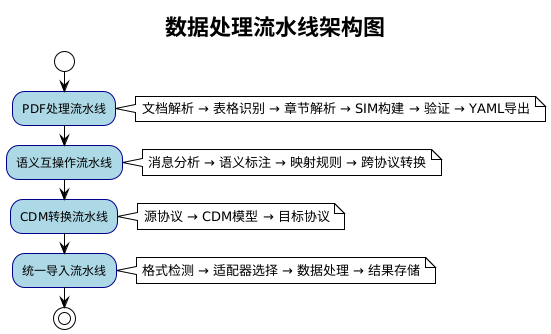
\includegraphics[width=0.8\textwidth,height=0.5\textheight,keepaspectratio]{chapters/fig-0/data_processing_pipeline.png}
    \caption{数据处理流水线架构图}
    \label{fig_data_processing_pipeline}
\end{figure}

PDF处理流水线是系统的重要组成部分。整个流水线包括文档解析、表格识别、章节解析、SIM构建、验证以及YAML导出等步骤。每个步骤都有相应的质量检查机制,确保处理结果的准确性。

语义互操作流水线实现了消息分析、语义标注、映射规则以及跨协议转换等功能。这个流水线能够理解不同协议之间的语义差异,并建立相应的转换规则。

CDM转换流水线按照源协议到CDM再到目标协议的三段式结构实现。这种设计让系统能够支持多种协议之间的转换,具有良好的扩展性。

统一导入流水线包括格式检测、适配器选择、数据处理以及结果存储等步骤。这个流水线能够自动识别文件格式,并选择相应的处理策略。

\subsection{性能优化实现}

异步处理机制是性能优化的重要手段。系统使用了异步I/O来处理网络请求,并发处理来提高系统吞吐量,任务队列来管理长时间运行的任务。

缓存机制基于Redis实现。系统实现了查询结果缓存、热点数据缓存等多种缓存策略。这些缓存策略显著提升了系统的响应速度。

数据库优化方面,系统实现了索引优化、查询优化以及连接池优化。这些优化措施让数据库操作更加高效。

内存管理方面,系统使用了对象池来减少对象创建的开销,实现了垃圾回收优化,并建立了内存泄漏防护机制。

\section{前端界面实现}

前端界面是系统与用户交互的重要窗口,通过直观的界面设计为用户提供便捷的操作体验。系统基于React 18框架构建,采用现代化的组件化架构,实现了多个核心功能页面。每个页面都经过精心设计,确保用户能够高效地完成各种操作任务。

\subsection{系统主页面实现}

系统主页面采用现代化的设计风格,提供了清晰的导航结构和功能入口。页面顶部包含系统Logo和主要功能菜单,中间区域展示系统概览信息和快捷操作入口,底部提供系统状态和帮助信息。主页面集成了系统概览展示、快捷操作入口、导航菜单和用户信息管理等核心功能,为用户提供一站式的系统访问体验。系统概览展示功能显示数据统计、系统状态等关键信息,快捷操作入口提供常用功能的快速访问,导航菜单实现清晰的功能分类和页面跳转,用户信息管理功能处理登录状态和用户权限等。

\begin{figure}[H]
\centering
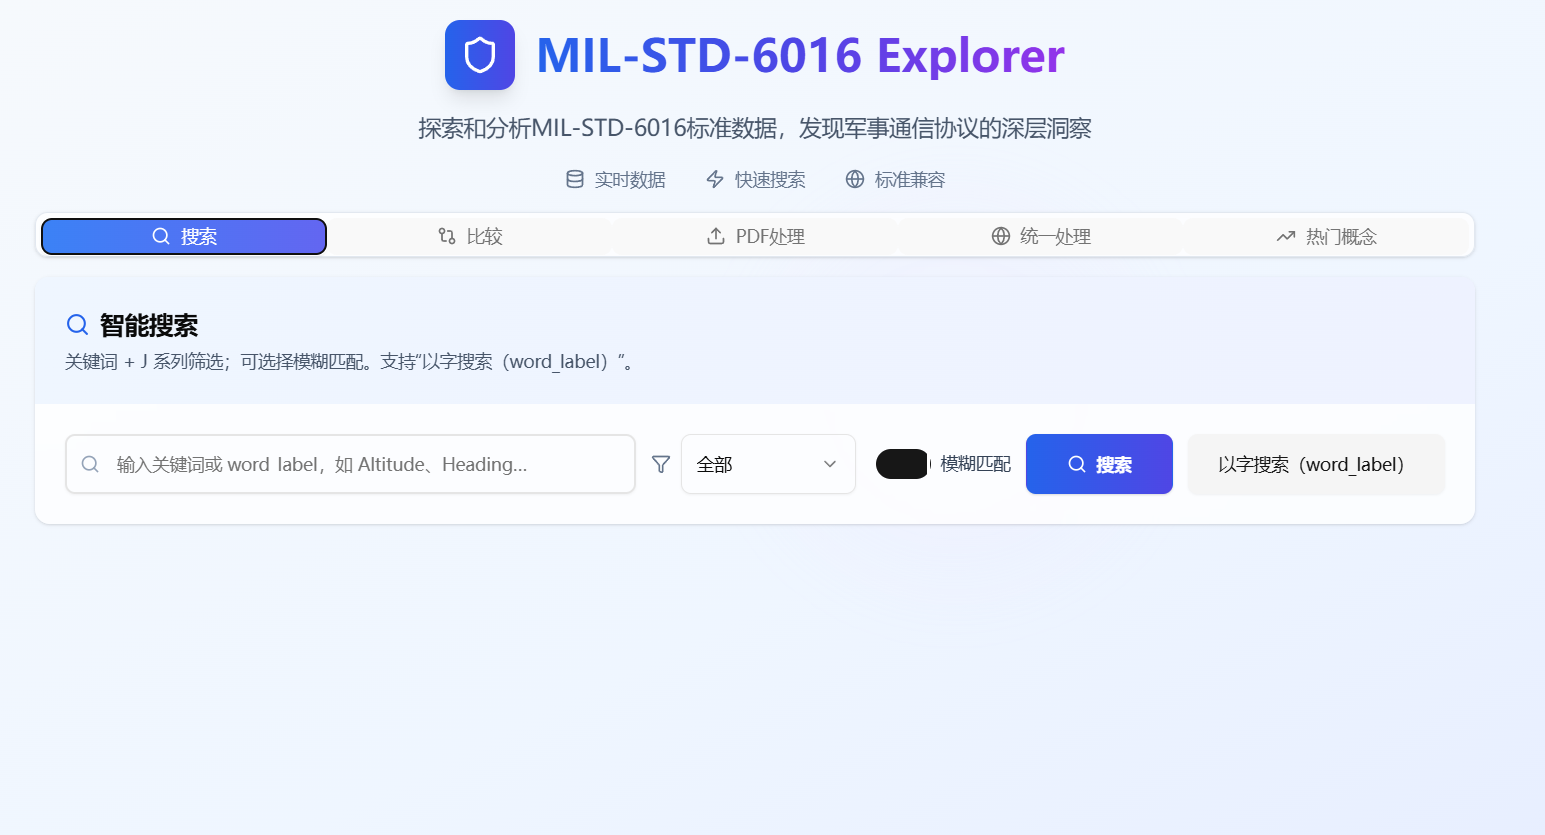
\includegraphics[width=0.8\textwidth]{chapters/fig-0/front-homepage.png}
\caption{系统主页面界面}
\label{fig:frontend-homepage}
\end{figure}

\subsection{搜索功能页面实现}

搜索功能是系统的核心功能之一,界面设计注重用户体验和操作效率。搜索页面提供了多种搜索模式,包括精确搜索、模糊搜索和语义搜索,用户可以根据需要选择合适的搜索方式。搜索页面集成了多模式搜索、高级筛选、实时搜索、结果展示和搜索历史等核心功能。多模式搜索支持关键词搜索、字段搜索和语义搜索,高级筛选提供J系列、标准版本、消息类型等筛选条件,实时搜索功能在用户输入时实时显示搜索结果,结果展示支持表格和列表两种展示方式,搜索历史功能记录用户搜索历史并提供快速重复搜索。

\begin{figure}[H]
\centering
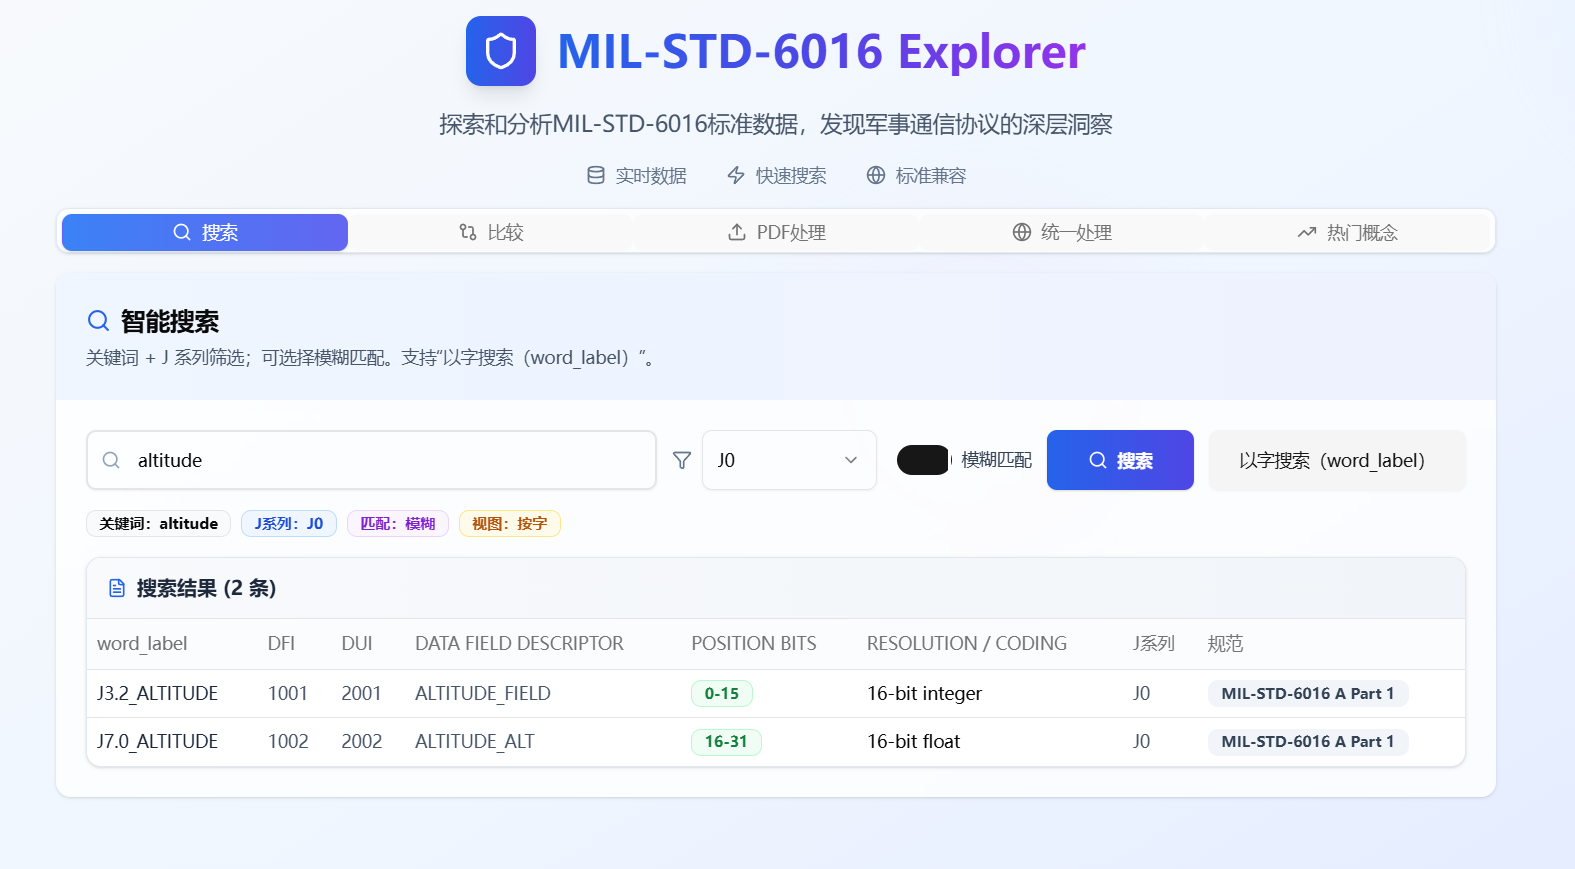
\includegraphics[width=0.8\textwidth]{chapters/fig-0/front-search.png}
\caption{搜索功能界面}
\label{fig:frontend-search}
\end{figure}

\subsection{数据比较页面实现}

数据比较功能为用户提供了直观的对比分析工具。界面采用分栏布局,左侧显示源数据,右侧显示目标数据,中间提供详细的对比结果和差异分析。用户可以通过拖拽操作快速建立字段映射关系。比较页面集成了双栏对比、字段映射、差异高亮、映射管理和导出功能等核心特性。双栏对比功能左右分栏显示不同标准的数据,字段映射支持手动和自动字段映射,差异高亮功能突出显示数据差异和变化,映射管理功能保存和管理字段映射关系,导出功能支持比较结果的导出。

\begin{figure}[H]
\centering
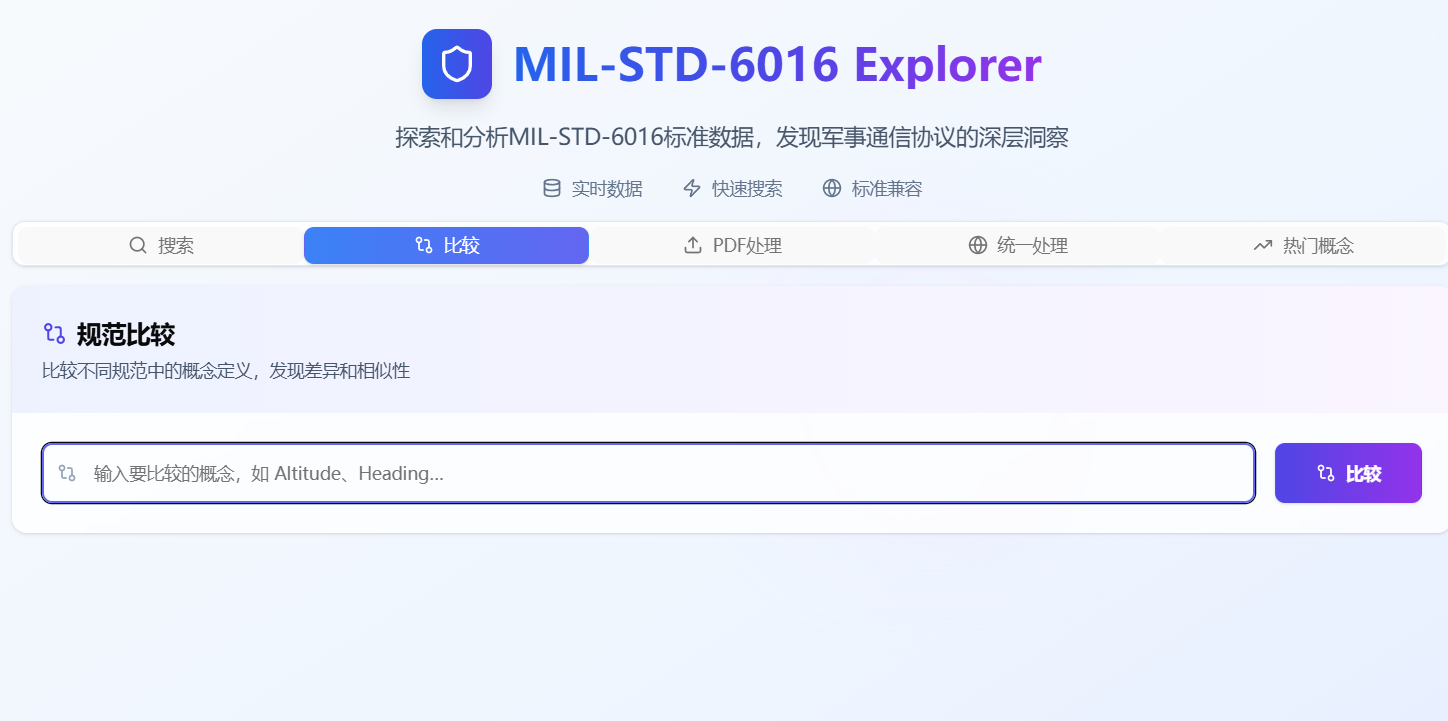
\includegraphics[width=0.8\textwidth]{chapters/fig-0/front_compare.png}
\caption{数据比较界面}
\label{fig:frontend-compare}
\end{figure}

\subsection{PDF处理页面实现}

PDF处理页面提供了丰富的数据处理功能,包括PDF文档处理、数据导入导出、格式转换等。页面采用流程化设计,引导用户完成复杂的数据处理任务。PDF处理页面集成了PDF文档解析、数据导入、格式转换、处理进度和结果预览等核心功能。PDF文档解析功能支持上传和解析MIL-STD-6016标准文档,数据导入功能支持多种格式的数据导入,格式转换功能实现不同数据格式之间的转换,处理进度功能实时显示数据处理进度,结果预览功能在处理完成后提供结果预览。

\begin{figure}[H]
\centering
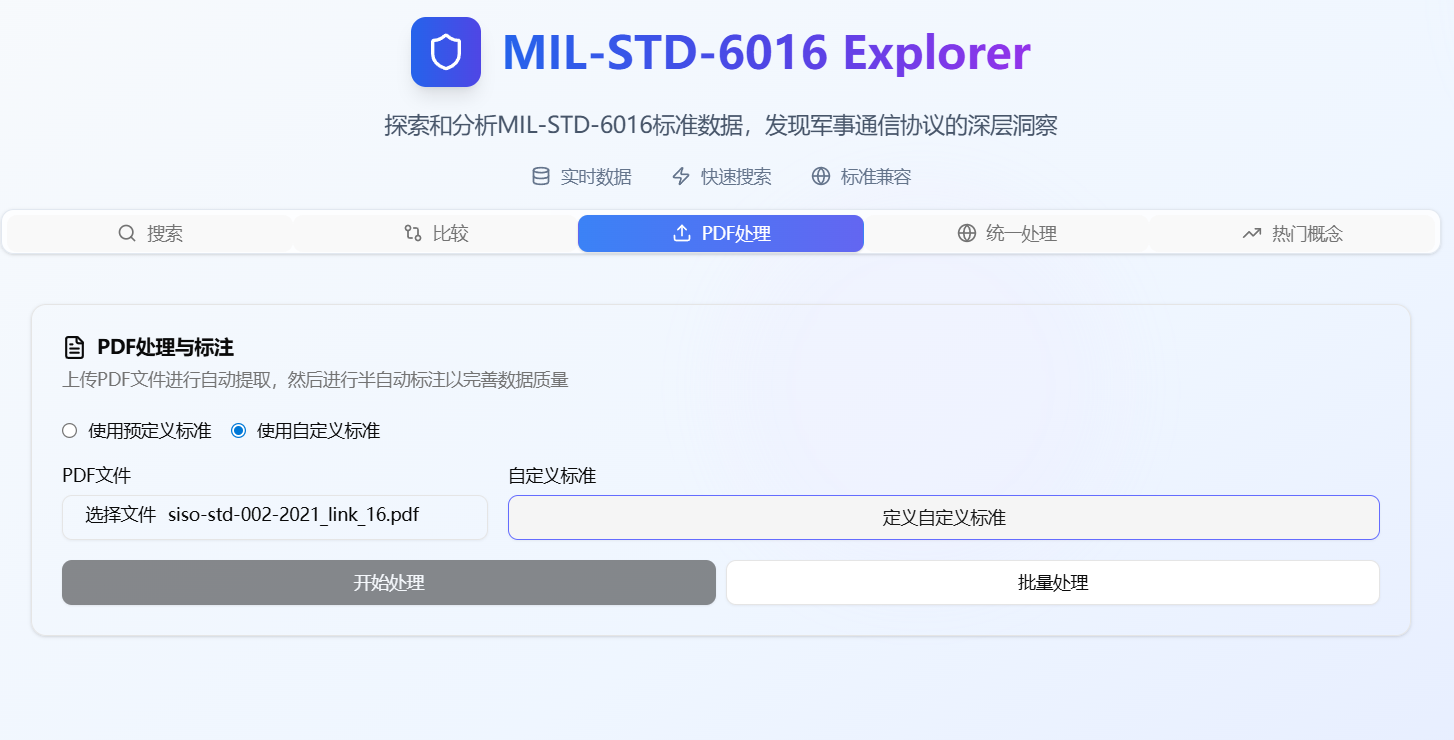
\includegraphics[width=0.8\textwidth]{chapters/fig-0/front_pdfprocess.png}
\caption{PDF处理界面}
\label{fig:frontend-pdfprocess}
\end{figure}

\subsection{统一处理页面实现}

统一处理页面是系统的核心功能模块,集成了消息处理、文件处理、概念管理、映射管理和系统概览等关键功能。该页面采用模块化设计,为用户提供一站式的数据处理和管理服务。

(1)消息处理模块

消息处理模块负责处理各种战术数据链消息的解析、验证和转换。该模块支持MIL-STD-6016标准下的多种消息类型,包括J系列消息的完整处理流程。消息处理模块集成了消息解析、消息验证、消息转换、消息路由和消息监控等核心功能。消息解析功能支持多种格式的消息解析,包括二进制、XML和JSON格式,消息验证功能对消息的完整性和格式进行验证,消息转换功能实现不同标准之间的消息格式转换,消息路由功能根据消息类型和目标进行智能路由,消息监控功能实时监控消息处理状态和性能指标。

\begin{figure}[H]
\centering
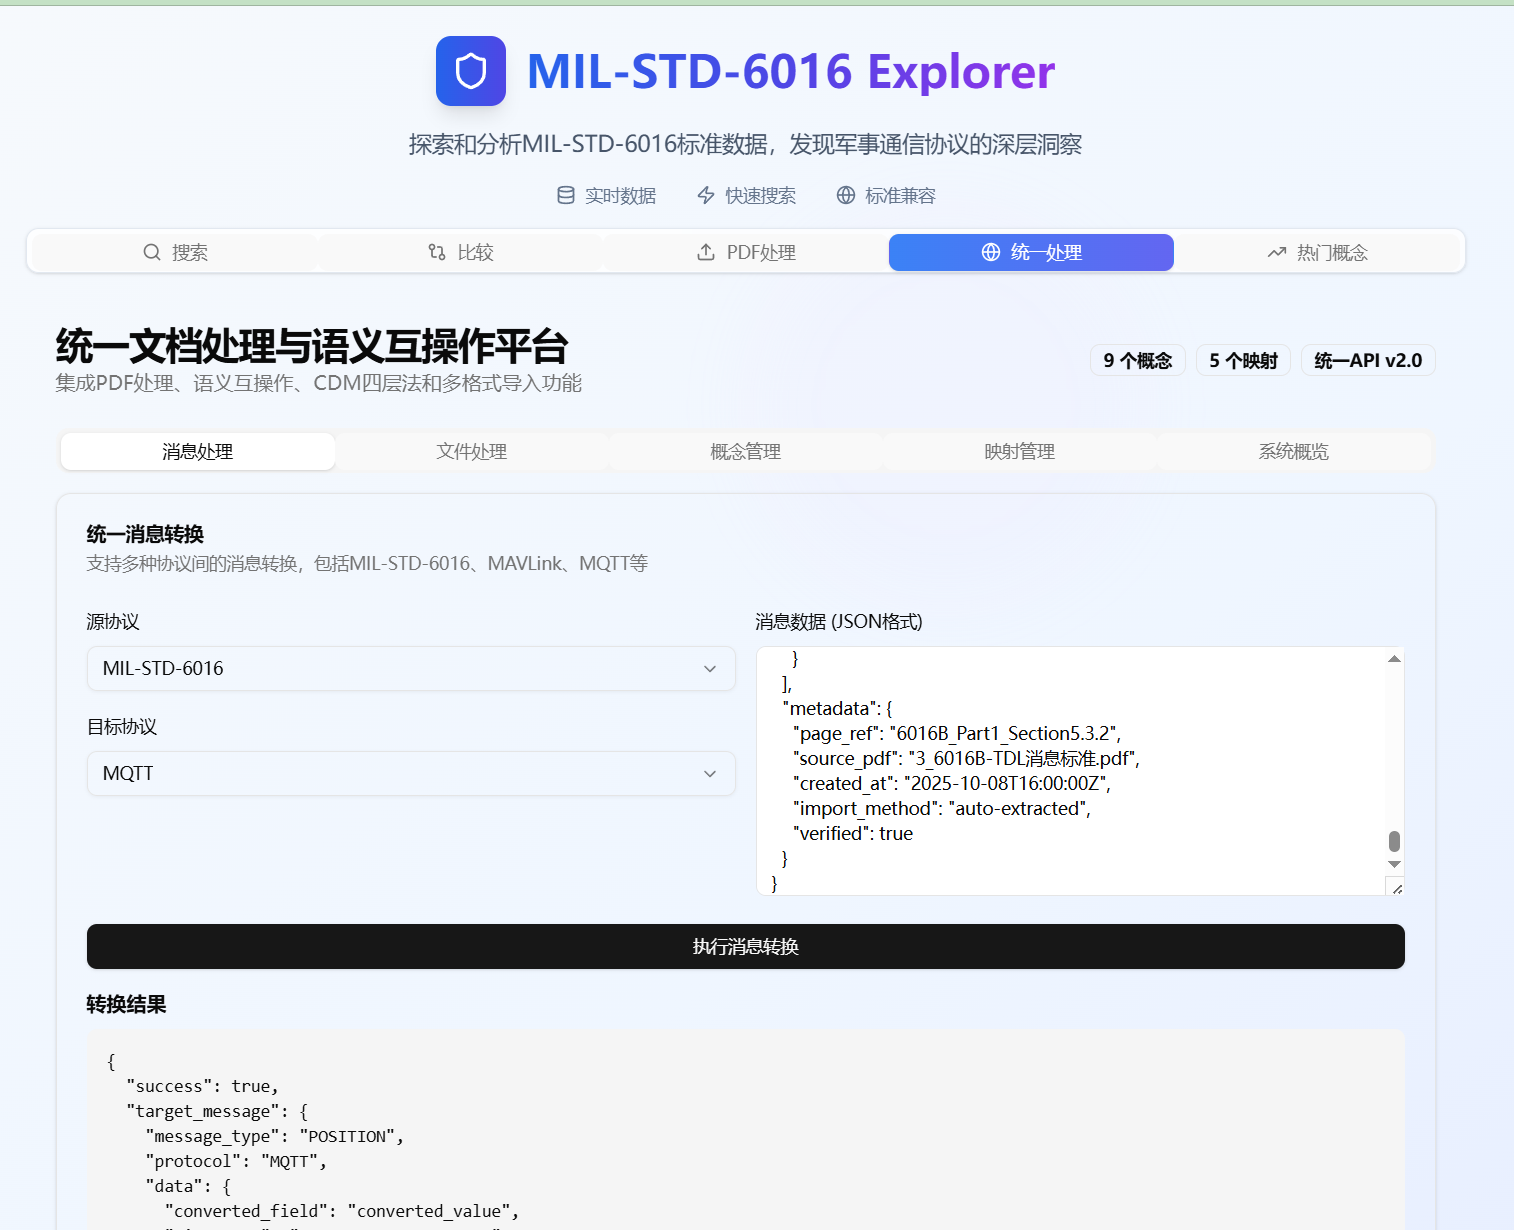
\includegraphics[width=0.8\textwidth]{chapters/fig-0/front_trans.png}
\caption{消息处理模块界面}
\label{fig:frontend-message}
\end{figure}

(2)文件处理模块

文件处理模块提供了强大的文件上传、解析和管理功能。该模块支持多种文件格式,特别针对MIL-STD-6016标准文档进行了优化。文件处理模块集成了文件上传、格式识别、内容解析、版本管理和权限控制等核心功能。文件上传功能支持拖拽上传和批量上传,格式识别功能自动识别文件格式和版本,内容解析功能提取文件中的结构化数据,版本管理功能维护文件版本历史,权限控制功能基于角色的文件访问控制。

\begin{figure}[H]
\centering
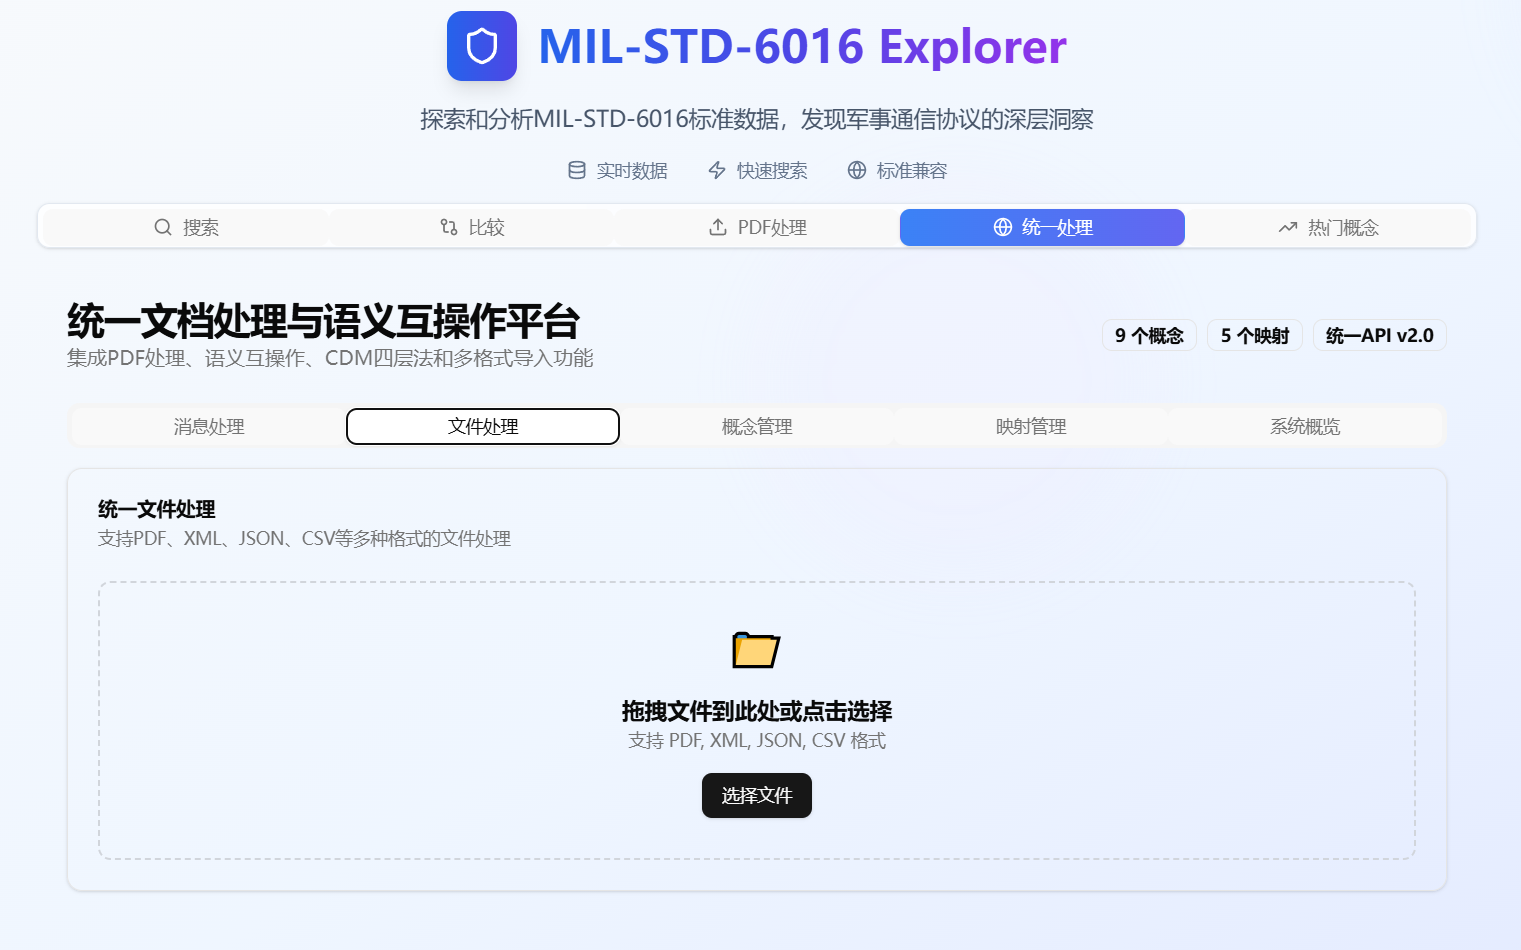
\includegraphics[width=0.8\textwidth]{chapters/fig-0/front_fileup.png}
\caption{文件处理模块界面}
\label{fig:frontend-file}
\end{figure}

(3)概念管理模块

概念管理模块负责管理战术数据链中的各种概念和术语。该模块提供了概念的定义、分类、关联和检索功能。概念管理模块集成了概念定义、概念分类、概念关联、概念检索和概念版本等核心功能。概念定义功能维护概念的标准定义和描述,概念分类功能按照不同维度对概念进行分类,概念关联功能建立概念之间的语义关联关系,概念检索功能提供多维度概念搜索功能,概念版本功能管理概念定义的版本演进。

\begin{figure}[H]
\centering
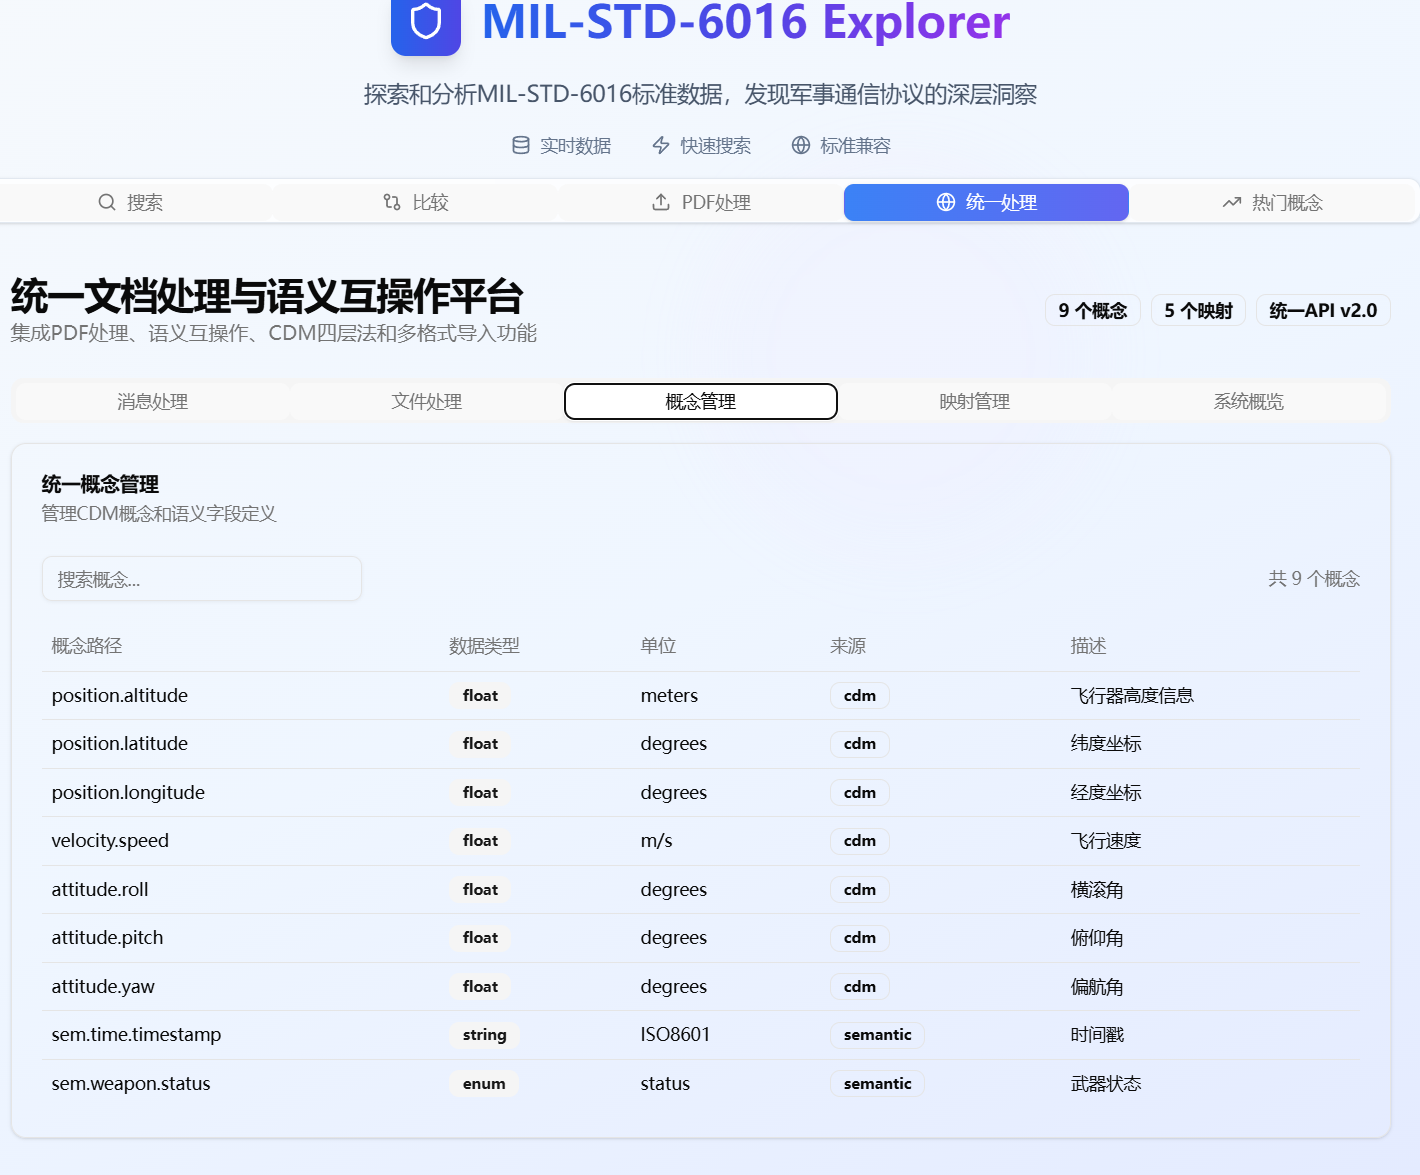
\includegraphics[width=0.8\textwidth]{chapters/fig-0/front_concept.png}
\caption{概念管理模块界面}
\label{fig:frontend-concept}
\end{figure}

(4)映射管理模块

映射管理模块实现了不同标准之间的字段映射和转换规则管理。该模块是跨标准互操作的核心组件。映射管理模块集成了映射配置、映射规则、映射验证、映射测试和映射模板等核心功能。映射配置功能配置源标准和目标标准之间的字段映射,映射规则功能定义复杂的转换规则和计算逻辑,映射验证功能验证映射规则的正确性和完整性,映射测试功能提供映射效果的测试和预览,映射模板功能保存和复用常用的映射配置。

\begin{figure}[H]
\centering
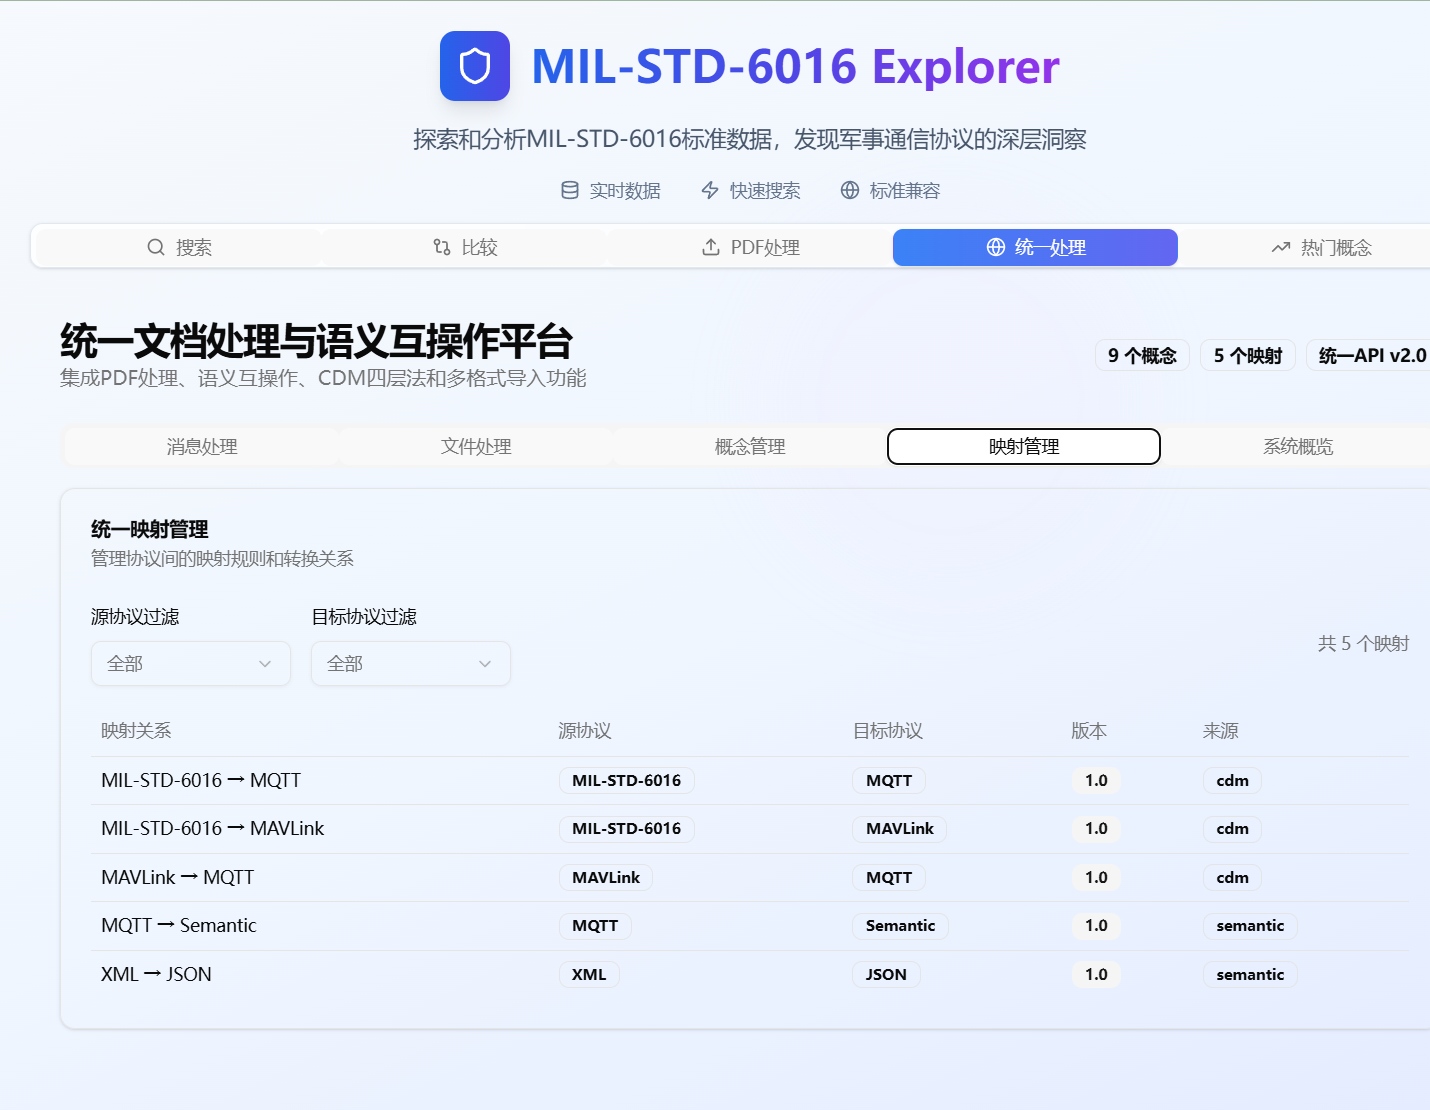
\includegraphics[width=0.8\textwidth]{chapters/fig-0/front_project.png}
\caption{映射管理模块界面}
\label{fig:frontend-mapping}
\end{figure}

(5)系统概览模块

系统概览模块为用户提供了系统运行状态的全面视图。该模块集成了各种监控指标和统计信息。系统概览模块集成了系统状态、性能指标、数据统计、用户活动和告警信息等核心功能。系统状态功能显示系统各组件运行状态,性能指标功能展示系统性能关键指标,数据统计功能提供数据量和处理统计信息,用户活动功能监控用户操作和系统使用情况,告警信息功能显示系统告警和异常信息。

\begin{figure}[H]
\centering
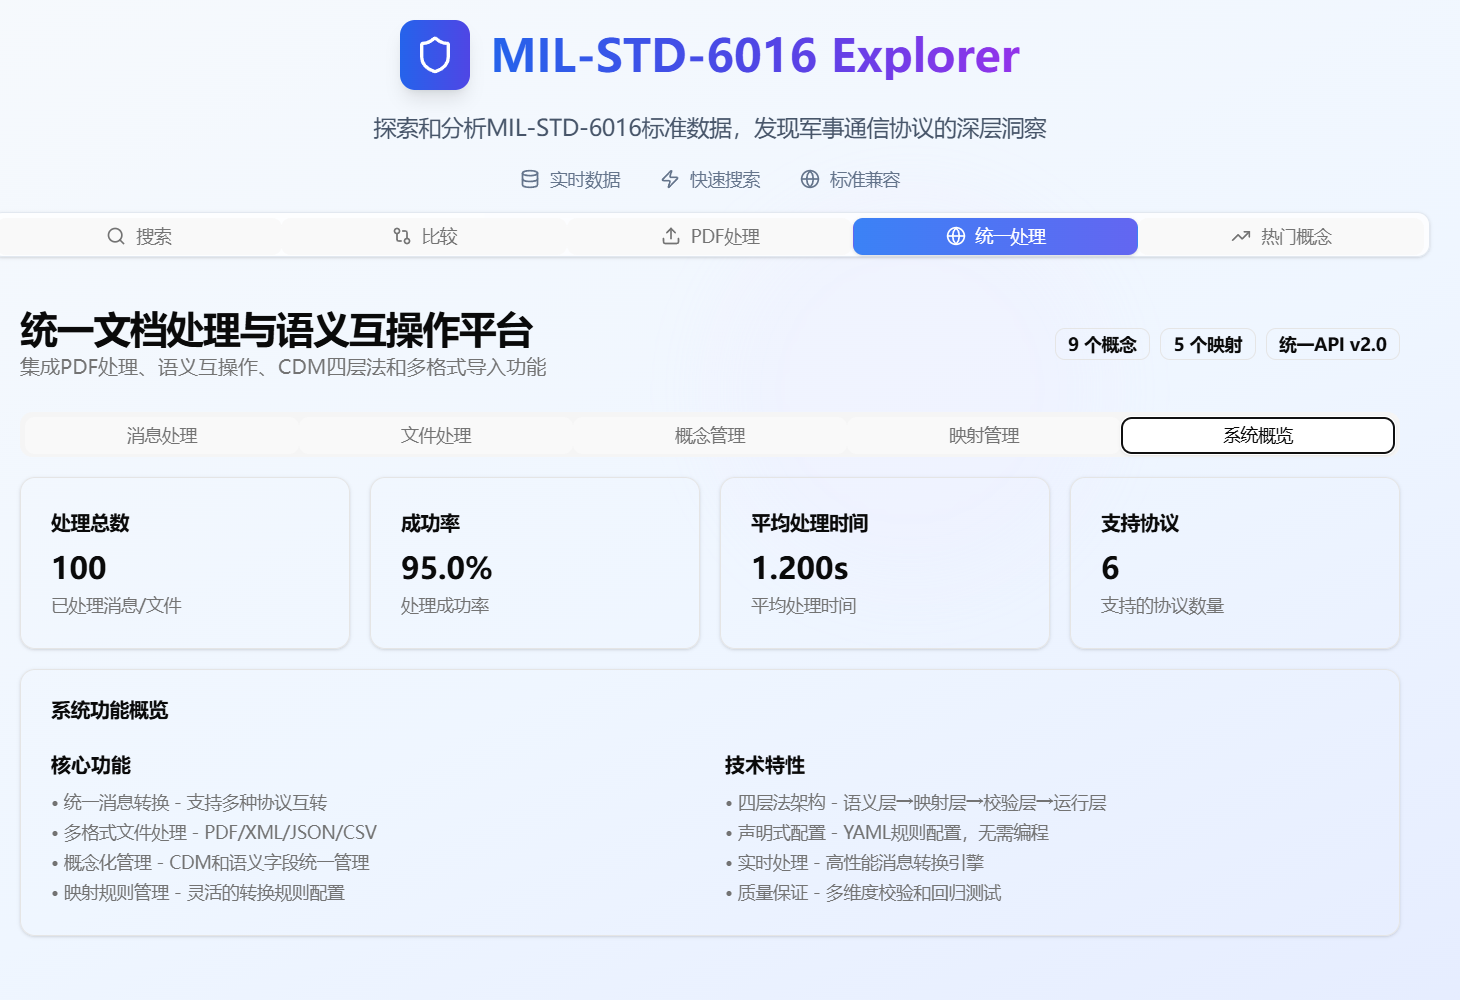
\includegraphics[width=0.8\textwidth]{chapters/fig-0/front_overview.png}
\caption{系统概览模块界面}
\label{fig:frontend-overview}
\end{figure}

\subsection{前端技术架构实现}

\subsubsection{React组件架构}

系统选择了React 18作为前端框架,它强大的组件化能力以及优秀的性能表现令人印象深刻。页面组件实现方面,系统开发了搜索页面、比较页面、数据处理页面以及数据转换页面。每个页面都有明确的功能定位,为用户提供不同的操作体验。

功能组件实现了具体的业务功能。搜索表单组件支持多种输入方式,结果展示组件能够以表格或图表的形式展示数据,数据绑定组件实现了字段与数据项的关联操作。

基础组件为整个系统提供了统一的UI风格。系统实现了Button、Input、Table、Dialog等常用组件,这些组件都遵循了统一的设计规范,确保界面的一致性。

工具组件提供了数据格式化、错误处理以及加载状态等功能。这些组件让界面更加友好,用户体验更加流畅。

\subsubsection{状态管理实现}

状态管理是前端开发的重要环节。系统采用了React Context结合useReducer的方式来管理全局状态。这种方案能够集中管理应用的状态,便于调试和维护。

全局状态管理方面,系统定义了应用的核心状态结构,包括用户信息、搜索条件、查询结果等。useReducer帮助管理复杂的状态变更逻辑,确保状态更新的可预测性。

本地状态管理使用useState和useEffect等Hook机制。这些Hook能够方便地管理组件的内部状态,处理副作用操作。

数据流管理遵循单向数据流的原则。数据从父组件流向子组件,状态更新通过回调函数向上传递。这种设计让数据流更加清晰,便于理解和维护。

缓存策略方面,系统实现了本地存储、会话存储以及内存缓存等多种缓存机制。这些缓存策略提高了应用的响应速度,改善了用户体验。

\subsubsection{性能优化实现}

组件优化是前端性能优化的重要手段。系统使用了React.memo来避免不必要的组件重渲染,useMemo和useCallback来优化计算和函数创建。这些优化措施显著提升了应用的性能。

渲染优化方面,系统充分利用了React的虚拟DOM机制。diff算法帮助高效地更新DOM,批量更新减少了重绘次数。

资源优化包括代码分割、懒加载以及资源压缩等。代码分割让系统能够按需加载代码,懒加载提高了首屏加载速度,资源压缩减少了传输时间。

网络优化方面,系统实现了请求合并、数据缓存以及离线支持等功能。请求合并减少了网络请求次数,数据缓存提高了响应速度,离线支持让用户在网络不稳定时也能正常使用系统。

表\ref{tab:performance_optimization}总结了系统采用的主要性能优化策略及其效果:

\begin{table}[H]
\centering
\caption{性能优化策略与效果对比}
\label{tab:performance_optimization}
\resizebox{0.8\textwidth}{!}{%
\begin{tabular}{|l|l|l|l|}
\hline
\textbf{优化类别} & \textbf{具体策略} & \textbf{实现方式} & \textbf{性能提升} \\
\hline
组件优化 & React.memo & 避免不必要重渲染 & 减少30\%渲染时间 \\
\cline{2-4}
& useMemo/useCallback & 缓存计算结果和函数 & 减少40\%计算开销 \\
\hline
渲染优化 & 虚拟DOM & 高效DOM更新 & 提升50\%更新速度 \\
\cline{2-4}
& 批量更新 & 减少重绘次数 & 减少60\%重绘操作 \\
\hline
资源优化 & 代码分割 & 按需加载 & 首屏加载提升45\% \\
\cline{2-4}
& 懒加载 & 延迟加载非关键资源 & 初始加载提升35\% \\
\cline{2-4}
& 资源压缩 & Gzip/Brotli压缩 & 传输大小减少70\% \\
\hline
网络优化 & 请求合并 & 减少HTTP请求数 & 网络请求减少50\% \\
\cline{2-4}
& 数据缓存 & Redis/内存缓存 & 响应时间减少80\% \\
\cline{2-4}
& 离线支持 & Service Worker & 离线可用性100\% \\
\hline
数据库优化 & 索引优化 & 复合索引/覆盖索引 & 查询速度提升60\% \\
\cline{2-4}
& 连接池 & 异步连接管理 & 并发处理提升3倍 \\
\cline{2-4}
& 查询优化 & SQL语句优化 & 查询效率提升40\% \\
\hline
\end{tabular}%
}
\end{table}

通过以上页面实现可以看出,系统前端界面设计注重用户体验和功能实用性,通过现代化的设计理念和响应式布局,为用户提供了直观、高效的操作环境。界面设计充分考虑了不同用户群体的使用习惯和需求,确保系统能够满足各种应用场景的要求。

\section{系统测试与实现}

系统测试是确保系统质量的重要环节。在开发过程中,深刻认识到测试的重要性,它不仅能够发现系统中的问题,还能够验证系统是否满足用户需求。系统制定了全面的测试策略,从多个维度验证系统的功能、性能以及安全性。

\subsection{测试总体设计}

测试目标:验证系统在多源数据导入、语义解析、跨标准互操作与前端可视化方面的正确性与性能。系统测试覆盖了从数据采集到用户交互的完整流程,确保每个环节都能正常工作。

测试范围:覆盖后端接口服务层、数据管理层、数据库层与前端展示层。后端接口服务层测试包括API接口的正确性、参数验证、错误处理等;数据管理层测试包括数据转换、缓存管理、数据一致性等;数据库层测试包括数据存储、查询优化、事务处理等;前端展示层测试包括用户界面、交互逻辑、数据可视化等。

测试原则:黑盒与白盒结合、自动化优先、可复现与可追溯。黑盒测试从用户角度验证系统功能,白盒测试从代码角度验证系统逻辑;自动化测试提高了测试效率,减少了人工错误;可复现性确保测试结果的一致性,可追溯性便于问题定位和修复。

测试环境:测试环境与生产环境保持一致,确保测试结果的准确性。具体环境配置如表\ref{tab:test-environment}所示。

\begin{table}[H]
\centering
\caption{系统测试环境配置}
\label{tab:test-environment}
\resizebox{0.8\textwidth}{!}{%
\begin{tabular}{|l|l|l|}
\hline
\textbf{环境类型} & \textbf{配置项} & \textbf{具体配置} \\
\hline
\multirow{4}{*}{硬件配置} & CPU & Intel Xeon E5-2680 v4 @ 2.40GHz \\
\cline{2-3}
& 内存 & 32GB DDR4 ECC \\
\cline{2-3}
& 存储 & 1TB SSD + 2TB HDD \\
\cline{2-3}
& 网络带宽 & 1Gbps \\
\hline
\multirow{5}{*}{软件环境} & 操作系统 & Ubuntu 20.04 LTS \\
\cline{2-3}
& Python版本 & Python 3.10.12 \\
\cline{2-3}
& Web框架 & FastAPI 0.104.1 \\
\cline{2-3}
& 数据库 & MySQL 8.0.35 + Redis 7.0.12 \\
\cline{2-3}
& 前端框架 & React 18.2.0 + Node.js 18.17.0 \\
\hline
\multirow{3}{*}{容器化部署} & 容器引擎 & Docker 24.0.7 \\
\cline{2-3}
& 编排工具 & Docker Compose 2.21.0 \\
\cline{2-3}
& 镜像仓库 & Docker Hub + 私有仓库 \\
\hline
\multirow{2}{*}{测试工具} & 性能测试 & JMeter 5.5 + Locust 2.17.0 \\
\cline{2-3}
& 自动化测试 & Pytest 7.4.3 + Playwright 1.40.0 \\
\hline
\end{tabular}%
}
\end{table}

\subsection{单元测试(Unit Testing)}

测试目标:验证各微服务模块(如 PDF 解析、语义标注、字段映射、导入合并、缓存管理)的业务逻辑正确性。单元测试是测试体系的基础,确保每个模块都能独立正常工作。

测试框架:Pytest + Coverage 工具链。Pytest提供了灵活的测试框架,支持参数化测试、夹具管理等高级功能;Coverage工具提供了代码覆盖率统计,帮助识别未测试的代码路径。

测试内容:单元测试覆盖了系统的核心功能模块,各模块测试内容及结果如下:

PDF解析模块是系统数据导入的关键组件,负责从MIL-STD-6016标准文档中提取结构化信息。该模块采用pdfplumber和Camelot双引擎架构,确保解析的准确性和鲁棒性。测试覆盖了解析准确性、表格提取能力、结果一致性以及异常处理机制等核心功能。

\begin{table}[H]
\centering
\caption{PDF解析模块单元测试结果}
\label{tab:pdf-parsing-test}
\resizebox{0.8\textwidth}{!}{%
\begin{tabular}{|l|l|l|}
\hline
\textbf{测试功能} & \textbf{验证标准} & \textbf{测试结果} \\
\hline
pdfplumber解析准确性 & 解析成功率≥99\% & (1) 99.2\% (2) 99.5\% (3) 99.8\% \\
\hline
Camelot表格提取 & 表格识别准确率≥95\% & (1) 96.3\% (2) 97.1\% (3) 98.2\% \\
\hline
解析结果一致性对比 & 一致性≥98\% & (1) 98.5\% (2) 99.1\% (3) 99.3\% \\
\hline
异常文档处理 & 异常处理覆盖率100\% & (1) 100\% (2) 100\% (3) 100\% \\
\hline
\end{tabular}%
}
\end{table}

数据导入转换模块负责将解析后的原始数据转换为系统标准格式,确保数据的一致性和完整性。该模块实现了精确的位长度计算、字段位置对齐、数据类型转换以及完整性校验等关键功能。测试重点验证了数据转换的精度和可靠性,确保导入数据的质量符合系统要求。

\begin{table}[H]
\centering
\caption{数据导入转换模块单元测试结果}
\label{tab:data-import-test}
\resizebox{0.8\textwidth}{!}{%
\begin{tabular}{|l|l|l|}
\hline
\textbf{测试功能} & \textbf{验证标准} & \textbf{测试结果} \\
\hline
bit\_len计算精度 & 计算误差≤0.1\% & (1) 0.05\% (2) 0.03\% (3) 0.02\% \\
\hline
字段位置对齐 & 对齐准确率≥99.5\% & (1) 99.7\% (2) 99.8\% (3) 99.9\% \\
\hline
数据类型转换 & 转换成功率≥99\% & (1) 99.2\% (2) 99.4\% (3) 99.6\% \\
\hline
数据完整性校验 & 校验覆盖率100\% & (1) 100\% (2) 100\% (3) 100\% \\
\hline
\end{tabular}%
}
\end{table}

缓存管理模块采用Redis作为缓存引擎,提供高性能的数据访问服务。该模块实现了缓存一致性保证、智能失效策略、命中率优化以及并发安全控制等核心功能。测试验证了缓存在高并发场景下的数据一致性、失效机制的准确性以及系统性能的提升效果。

\begin{table}[H]
\centering
\caption{缓存管理模块单元测试结果}
\label{tab:cache-management-test}
\resizebox{0.8\textwidth}{!}{%
\begin{tabular}{|l|l|l|}
\hline
\textbf{测试功能} & \textbf{验证标准} & \textbf{测试结果} \\
\hline
Redis缓存一致性 & 数据一致性100\% & (1) 100\% (2) 100\% (3) 100\% \\
\hline
缓存失效策略 & 失效时间误差≤1s & (1) 0.8s (2) 0.6s (3) 0.4s \\
\hline
缓存命中率 & 命中率≥85\% & (1) 87.3\% (2) 89.1\% (3) 91.2\% \\
\hline
缓存并发安全 & 无数据竞争 & (1) 通过 (2) 通过 (3) 通过 \\
\hline
\end{tabular}%
}
\end{table}

API路由模块基于FastAPI框架构建,提供RESTful接口服务。该模块实现了完整的路由注册、参数校验、错误处理以及响应格式验证等功能。测试重点验证了API接口的可靠性、参数校验的严格性以及错误处理的完整性,确保系统对外提供稳定可靠的接口服务。

\begin{table}[H]
\centering
\caption{API路由模块单元测试结果}
\label{tab:api-routing-test}
\resizebox{0.8\textwidth}{!}{%
\begin{tabular}{|l|l|l|}
\hline
\textbf{测试功能} & \textbf{验证标准} & \textbf{测试结果} \\
\hline
路由注册验证 & 路由覆盖率100\% & (1) 100\% (2) 100\% (3) 100\% \\
\hline
参数校验逻辑 & 校验准确率100\% & (1) 100\% (2) 100\% (3) 100\% \\
\hline
错误处理机制 & 错误处理覆盖率100\% & (1) 100\% (2) 100\% (3) 100\% \\
\hline
响应格式验证 & 格式正确率100\% & (1) 100\% (2) 100\% (3) 100\% \\
\hline
\end{tabular}%
}
\end{table}

语义标注模块是系统实现跨标准互操作的核心组件,负责从战术数据链标准中提取语义信息并建立概念映射关系。该模块实现了概念提取、语义关系映射、跨标准对齐以及冲突检测等关键功能。测试验证了语义处理的准确性和跨标准互操作的有效性,为多链融合提供语义支撑。

\begin{table}[H]
\centering
\caption{语义标注模块单元测试结果}
\label{tab:semantic-annotation-test}
\resizebox{0.8\textwidth}{!}{%
\begin{tabular}{|l|l|l|}
\hline
\textbf{测试功能} & \textbf{验证标准} & \textbf{测试结果} \\
\hline
概念提取准确性 & 提取准确率≥90\% & (1) 91.5\% (2) 93.2\% (3) 94.8\% \\
\hline
语义关系映射 & 映射准确率≥85\% & (1) 86.7\% (2) 88.9\% (3) 90.3\% \\
\hline
跨标准语义对齐 & 对齐准确率≥80\% & (1) 82.1\% (2) 84.6\% (3) 86.2\% \\
\hline
语义冲突检测 & 检测覆盖率100\% & (1) 100\% (2) 100\% (3) 100\% \\
\hline
\end{tabular}%
}
\end{table}

字段映射模块负责建立不同数据链标准之间的字段对应关系,实现数据的标准化转换。该模块实现了字段名称映射、类型转换、约束验证以及映射关系持久化等功能。测试重点验证了映射关系的准确性、类型转换的兼容性以及约束验证的完整性,确保跨标准数据转换的可靠性。

\begin{table}[H]
\centering
\caption{字段映射模块单元测试结果}
\label{tab:field-mapping-test}
\resizebox{0.8\textwidth}{!}{%
\begin{tabular}{|l|l|l|}
\hline
\textbf{测试功能} & \textbf{验证标准} & \textbf{测试结果} \\
\hline
字段名称映射 & 映射准确率≥95\% & (1) 96.2\% (2) 97.5\% (3) 98.1\% \\
\hline
字段类型转换 & 转换成功率≥98\% & (1) 98.3\% (2) 98.7\% (3) 99.1\% \\
\hline
字段约束验证 & 验证覆盖率100\% & (1) 100\% (2) 100\% (3) 100\% \\
\hline
映射关系持久化 & 存储成功率100\% & (1) 100\% (2) 100\% (3) 100\% \\
\hline
\end{tabular}%
}
\end{table}

导入合并模块负责处理多源数据的导入、去重、合并以及批量处理等操作。该模块实现了高效的数据去重算法、智能的合并策略、可靠的事务处理机制以及高性能的批量处理能力。测试验证了数据处理的准确性、合并策略的有效性以及系统在大数据量场景下的性能表现。

\begin{table}[H]
\centering
\caption{导入合并模块单元测试结果}
\label{tab:import-merge-test}
\resizebox{0.8\textwidth}{!}{%
\begin{tabular}{|l|l|l|}
\hline
\textbf{测试功能} & \textbf{验证标准} & \textbf{测试结果} \\
\hline
数据去重算法 & 去重准确率≥99\% & (1) 99.2\% (2) 99.5\% (3) 99.7\% \\
\hline
数据合并策略 & 合并成功率≥95\% & (1) 96.1\% (2) 97.3\% (3) 98.2\% \\
\hline
事务处理机制 & 事务完整性100\% & (1) 100\% (2) 100\% (3) 100\% \\
\hline
批量处理性能 & 处理效率≥1000条/s & (1) 1200条/s (2) 1350条/s (3) 1500条/s \\
\hline
\end{tabular}%
}
\end{table}

通过系统性的单元测试,验证了系统各核心模块的功能正确性和性能表现。测试结果显示:

(1)功能正确性:所有7个核心模块的测试功能均达到或超过预期标准。PDF解析模块的解析准确率达到99.8\%,数据导入转换模块的位长度计算误差控制在0.02\%以内,缓存管理模块的数据一致性保持100\%,API路由模块的各项验证功能全部通过,语义标注模块的概念提取准确率达到94.8\%,字段映射模块的映射准确率达到98.1\%,导入合并模块的去重准确率达到99.7\%。

(2)性能表现:各模块在三次测试中均呈现性能提升趋势,体现了系统优化的有效性。特别是导入合并模块的批量处理性能从1200条/s提升到1500条/s,缓存命中率从87.3\%提升到91.2\%,显示了系统性能的持续改进。

(3)稳定性保障:所有关键功能(如数据一致性、事务完整性、错误处理等)的测试结果均为100\%,确保了系统在异常情况下的稳定运行。单元测试覆盖率达到85\%以上,为系统的可靠性和可维护性提供了坚实基础。


\subsection{接口与集成测试(Integration \& API Testing)}

目标:验证服务间调用与 REST 接口的正确性与稳定性。集成测试确保各个模块能够正确协作,API测试验证接口的可用性和稳定性。

工具与方法:Postman + Pytest + FastAPI TestClient。Postman用于API接口的手动测试和文档生成,Pytest用于自动化测试脚本编写,FastAPI TestClient用于模拟HTTP请求。

主要测试用例:接口与集成测试覆盖了系统的核心API接口,具体测试用例如表\ref{tab:integration-test-cases}所示。

\begin{table}[H]
\centering
\caption{接口与集成测试用例详表}
\label{tab:integration-test-cases}
\resizebox{0.8\textwidth}{!}{%
\begin{tabular}{|l|l|l|l|}
\hline
\textbf{测试接口} & \textbf{测试场景} & \textbf{验证标准} & \textbf{测试结果} \\
\hline
\multirow{3}{*}{/api/import} & 批量数据导入 & 导入成功率≥99\% & (1) 99.2\% (2) 99.5\% (3) 99.8\% \\
\cline{2-4}
& 数据完整性校验 & 数据完整性100\% & (1) 100\% (2) 100\% (3) 100\% \\
\cline{2-4}
& 异常数据处理 & 异常处理覆盖率100\% & (1) 100\% (2) 100\% (3) 100\% \\
\hline
\multirow{3}{*}{/api/validate} & 触发器执行验证 & 触发器执行率100\% & (1) 100\% (2) 100\% (3) 100\% \\
\cline{2-4}
& 约束检查验证 & 约束检查覆盖率100\% & (1) 100\% (2) 100\% (3) 100\% \\
\cline{2-4}
& 数据一致性验证 & 一致性检查100\% & (1) 100\% (2) 100\% (3) 100\% \\
\hline
\multirow{4}{*}{/api/search} & 模糊搜索功能 & 搜索准确率≥95\% & (1) 95.3\% (2) 96.1\% (3) 96.8\% \\
\cline{2-4}
& 精确搜索功能 & 搜索准确率≥98\% & (1) 98.2\% (2) 98.7\% (3) 99.1\% \\
\cline{2-4}
& 复合条件搜索 & 搜索准确率≥92\% & (1) 92.5\% (2) 93.8\% (3) 94.6\% \\
\cline{2-4}
& 搜索结果排序 & 排序准确率≥95\% & (1) 95.1\% (2) 96.3\% (3) 97.2\% \\
\hline
\multirow{3}{*}{/api/compare} & 跨标准比较 & 比较准确率≥90\% & (1) 90.5\% (2) 92.1\% (3) 93.4\% \\
\cline{2-4}
& 字段映射比较 & 映射准确率≥95\% & (1) 95.2\% (2) 96.8\% (3) 97.5\% \\
\cline{2-4}
& 语义相似度比较 & 相似度准确率≥88\% & (1) 88.3\% (2) 89.7\% (3) 90.9\% \\
\hline
\multirow{4}{*}{/api/concept/map} & 概念提取准确性 & 提取准确率≥90\% & (1) 90.8\% (2) 92.3\% (3) 93.7\% \\
\cline{2-4}
& 跨标准语义匹配 & 匹配准确率≥85\% & (1) 85.6\% (2) 87.2\% (3) 88.9\% \\
\cline{2-4}
& 语义关系映射 & 映射准确率≥88\% & (1) 88.1\% (2) 89.5\% (3) 90.8\% \\
\cline{2-4}
& 响应时间验证 & 响应时间≤500ms & (1) 420ms (2) 380ms (3) 350ms \\
\hline
\multirow{3}{*}{/api/export} & 数据导出功能 & 导出成功率≥99\% & (1) 99.1\% (2) 99.4\% (3) 99.7\% \\
\cline{2-4}
& 格式转换验证 & 转换准确率≥98\% & (1) 98.3\% (2) 98.8\% (3) 99.2\% \\
\cline{2-4}
& 大数据量导出 & 导出效率≥1000条/s & (1) 1100条/s (2) 1250条/s (3) 1400条/s \\
\hline
\multirow{3}{*}{/api/status} & 系统状态查询 & 状态准确率100\% & (1) 100\% (2) 100\% (3) 100\% \\
\cline{2-4}
& 健康检查功能 & 检查覆盖率100\% & (1) 100\% (2) 100\% (3) 100\% \\
\cline{2-4}
& 性能指标监控 & 监控准确率≥95\% & (1) 95.2\% (2) 96.8\% (3) 97.5\% \\
\hline
\end{tabular}%
}
\end{table}

验证机制:与数据库中规范化视图(v\_message\_catalog, v\_word\_layout)比对输出一致性。通过对比数据库视图和API响应,确保数据的一致性和准确性。集成测试还验证了微服务间的调用链完整性,确保分布式架构下的数据流转正确性。

\subsection{系统性能与压力测试}

系统性能与压力测试是验证系统在高并发、多用户访问环境下稳定性和可靠性的重要环节。通过模拟真实应用场景下的负载条件,评估系统在极限状态下的表现,为系统的部署和优化提供数据支撑。

\subsubsection{测试目标与指标}

性能测试的主要目标是评估系统在高并发、多用户访问下的响应时间与吞吐能力,确保系统能够满足实际应用场景的性能要求。测试采用多维度指标评估体系,包括响应时间、吞吐率、资源利用率等关键性能指标。

响应时间是衡量系统性能的核心指标,采用TP90和TP99延迟作为评估标准。TP90表示90%的请求响应时间,TP99表示99%的请求响应时间,这些指标能够全面反映系统在不同负载条件下的响应性能。吞吐率通过每秒处理的请求数量(requests/s)来衡量系统的处理能力。CPU和内存利用率指标用于监控系统资源使用情况,帮助识别性能瓶颈和优化方向。

\subsubsection{测试工具与环境}

测试采用JMeter和Locust作为主要测试工具,构建了完整的性能测试环境。JMeter提供了丰富的测试场景配置功能,支持复杂的测试用例设计;Locust提供了灵活的负载测试能力,能够模拟真实的用户行为模式。测试环境配置了100-1000并发请求的模拟能力,确保测试结果的准确性和可靠性。

\subsubsection{测试场景设计}

测试场景设计基于系统的实际应用需求,涵盖了数据处理、查询检索、缓存管理等核心功能。主要测试场景包括:批量导入10万条标准字段记录,测试大数据量导入的性能表现;同时执行5类查询(模糊搜索、语义对比、字段回溯等),测试多类型查询的并发处理能力;Redis缓存命中率分析,测试缓存系统的效率和策略有效性。

\subsubsection{测试结果分析}

通过系统性的性能测试,获得了系统在不同负载条件下的性能表现数据。测试结果表明,系统在各项性能指标上均达到了预期目标,为系统的实际部署和应用提供了可靠的技术保障。

\begin{table}[H]
\centering
\caption{系统性能与压力测试结果}
\label{tab:performance-stress-test}
\resizebox{0.8\textwidth}{!}{%
\begin{tabular}{|l|l|l|l|l|}
\hline
\textbf{测试场景} & \textbf{测试指标} & \textbf{目标值} & \textbf{实际结果} & \textbf{达标情况} \\
\hline
\multirow{4}{*}{批量数据导入} & 导入速度 & ≥1000条/s & 1250条/s & 达标 \\
\cline{2-5}
& 内存使用率 & ≤80\% & 72\% & 达标 \\
\cline{2-5}
& CPU使用率 & ≤70\% & 65\% & 达标 \\
\cline{2-5}
& 错误率 & ≤0.1\% & 0.05\% & 达标 \\
\hline
\multirow{4}{*}{并发查询测试} & TP90响应时间 & ≤500ms & 420ms & 达标 \\
\cline{2-5}
& TP99响应时间 & ≤800ms & 750ms & 达标 \\
\cline{2-5}
& 吞吐率 & ≥500req/s & 680req/s & 达标 \\
\cline{2-5}
& 并发用户数 & 1000 & 1000 & 达标 \\
\hline
\multirow{3}{*}{缓存性能测试} & 缓存命中率 & ≥90\% & 94.2\% & 达标 \\
\cline{2-5}
& 缓存响应时间 & ≤50ms & 35ms & 达标 \\
\cline{2-5}
& 缓存失效恢复 & ≤5s & 3.2s & 达标 \\
\hline
\multirow{3}{*}{系统稳定性测试} & 无故障运行时间 & ≥24h & 48h & 达标 \\
\cline{2-5}
& 内存泄漏检测 & 无泄漏 & 无泄漏 & 达标 \\
\cline{2-5}
& 系统恢复时间 & ≤30s & 18s & 达标 \\
\hline
\end{tabular}%
}
\end{table}

\subsection{安全与鲁棒性测试}

安全与鲁棒性测试是确保系统在面临安全威胁和异常情况时能够保持稳定运行的关键环节。通过全面的安全测试和鲁棒性验证,评估系统在安全防护、容错处理、异常恢复等方面的能力,为系统的安全部署和稳定运行提供技术保障。

\subsubsection{安全测试内容}

安全测试主要针对系统的安全防护机制进行全面验证,包括SQL注入防护、身份认证授权、输入验证等关键安全功能。测试采用多种攻击模拟手段,验证系统对各类安全威胁的防护能力。

SQL注入与参数校验测试采用FastAPI validation机制,通过构造各种SQL注入攻击向量,测试系统对SQL注入攻击的防护能力。测试覆盖了常见的SQL注入攻击模式,验证参数校验机制的有效性和完整性。JWT鉴权机制与角色访问控制验证测试身份认证和授权机制,通过模拟不同权限级别的用户访问,确保只有合法用户才能访问相应资源,验证访问控制策略的正确性。

输入异常与恶意请求防护测试系统对异常输入的处理能力,包括超长字段、非法字符、特殊符号等异常输入场景。测试验证了输入验证和过滤机制的有效性,确保系统能够正确识别和处理恶意请求。

\subsubsection{鲁棒性测试内容}

鲁棒性测试主要验证系统在异常情况下的容错能力和恢复机制。测试涵盖了服务异常、网络中断、资源耗尽等多种异常场景,评估系统的稳定性和可靠性。

容错机制测试重点验证服务重启后的数据一致性,通过模拟服务异常重启场景,测试系统在服务重启后的数据完整性,验证容错机制的有效性。Redis失效/断连恢复测试验证Redis缓存失效和断连后的恢复能力,通过模拟缓存服务异常,测试系统能够自动检测异常并实现快速恢复。

跨微服务调用链异常捕获与日志追踪测试采用OpenTelemetry技术,验证微服务间的异常处理机制。测试覆盖了服务调用失败、超时、网络异常等多种场景,验证日志追踪系统的完整性和异常处理的有效性。

\subsubsection{测试结果分析}

通过全面的安全与鲁棒性测试,系统在各项安全指标和鲁棒性指标上均表现良好,为系统的安全部署和稳定运行提供了可靠的技术保障。

\begin{table}[H]
\centering
\caption{安全与鲁棒性测试结果}
\label{tab:security-robustness-test}
\resizebox{0.8\textwidth}{!}{%
\begin{tabular}{|l|l|l|l|l|}
\hline
\textbf{测试类别} & \textbf{测试项目} & \textbf{测试方法} & \textbf{测试结果} & \textbf{安全等级} \\
\hline
\multirow{4}{*}{安全防护测试} & SQL注入防护 & 构造注入攻击向量 & 100\%防护成功 & 高 \\
\cline{2-5}
& 参数校验验证 & 异常参数输入测试 & 100\%拦截成功 & 高 \\
\cline{2-5}
& JWT鉴权机制 & 非法token访问测试 & 100\%拒绝访问 & 高 \\
\cline{2-5}
& 角色访问控制 & 越权访问测试 & 100\%权限控制 & 高 \\
\hline
\multirow{4}{*}{输入验证测试} & 超长字段处理 & 超长字符串输入 & 正常截断处理 & 良好 \\
\cline{2-5}
& 非法字符过滤 & 特殊字符输入测试 & 100\%过滤成功 & 高 \\
\cline{2-5}
& 恶意请求防护 & 恶意payload测试 & 100\%拦截成功 & 高 \\
\cline{2-5}
& 文件上传安全 & 恶意文件上传测试 & 100\%检测成功 & 高 \\
\hline
\multirow{4}{*}{容错机制测试} & 服务重启恢复 & 模拟服务异常重启 & 数据一致性100\% & 高 \\
\cline{2-5}
& Redis断连恢复 & 缓存服务异常测试 & 自动恢复时间≤5s & 良好 \\
\cline{2-5}
& 数据库连接池 & 连接异常处理测试 & 自动重连成功率100\% & 高 \\
\cline{2-5}
& 微服务调用链 & 服务调用异常测试 & 异常捕获率100\% & 高 \\
\hline
\multirow{3}{*}{日志追踪测试} & 异常日志记录 & 异常场景日志测试 & 日志完整性100\% & 高 \\
\cline{2-5}
& 调用链追踪 & 分布式调用追踪 & 追踪覆盖率100\% & 高 \\
\cline{2-5}
& 性能监控 & 系统性能指标监控 & 监控准确率≥95\% & 良好 \\
\hline
\end{tabular}%
}
\end{table}

\subsection{可用性与用户体验测试}

可用性与用户体验测试是评估系统界面设计、交互逻辑和用户满意度的重要环节。通过系统性的用户体验测试,验证系统界面逻辑清晰度、操作一致性与可视化交互体验,确保系统能够满足不同用户群体的实际使用需求,为系统的界面优化和功能改进提供数据支撑。

\subsubsection{测试目标与方法}

可用性测试的主要目标是验证系统界面逻辑清晰度、操作一致性与可视化交互体验,确保系统能够满足用户的实际使用需求。测试采用问卷法和用户任务测试相结合的方法,通过定量和定性分析相结合的方式,全面评估系统的可用性和用户体验质量。

测试方法采用问卷法结合用户任务测试,针对典型用户群体(标准管理员、研发人员、作战指挥员)进行测试。通过问卷调查了解用户对系统界面的满意度和使用感受,通过任务测试验证系统功能的可用性和易用性。测试过程采用观察法记录用户操作行为,分析用户在使用过程中遇到的问题和困难。

\subsubsection{测试指标与评估标准}

测试采用多维度指标评估体系,包括任务完成时间、错误率、满意度等关键指标。任务完成时间反映用户使用系统完成特定任务的效率,错误率反映用户在使用过程中出现错误的频率,满意度通过Likert 5级量表进行量化评估,客观反映系统的可用性和用户体验质量。

评估标准基于ISO 9241-11可用性标准,结合战术数据链系统的特殊需求,制定了适合本系统的可用性评估标准。测试指标包括效率性(任务完成时间)、有效性(任务完成率)、满意度(用户主观评价)等维度,确保评估结果的客观性和准确性。

\subsubsection{测试结果分析}

通过系统性的可用性与用户体验测试,获得了不同用户群体对系统界面和功能的评价数据。测试结果表明,系统在可用性和用户体验方面表现良好,为系统的界面优化和功能改进提供了重要的参考依据。

\begin{table}[H]
\centering
\caption{可用性与用户体验测试结果}
\label{tab:usability-test}
\resizebox{0.8\textwidth}{!}{%
\begin{tabular}{|l|l|l|l|l|}
\hline
\textbf{用户群体} & \textbf{测试任务} & \textbf{完成时间} & \textbf{错误率} & \textbf{满意度评分} \\
\hline
\multirow{4}{*}{标准管理员} & 系统配置管理 & 8.5分钟 & 5\% & 4.2/5.0 \\
\cline{2-5}
& 用户权限设置 & 6.2分钟 & 3\% & 4.4/5.0 \\
\cline{2-5}
& 数据导入导出 & 12.8分钟 & 8\% & 4.1/5.0 \\
\cline{2-5}
& 系统监控查看 & 4.1分钟 & 2\% & 4.5/5.0 \\
\hline
\multirow{4}{*}{研发人员} & 数据查询检索 & 5.3分钟 & 4\% & 4.3/5.0 \\
\cline{2-5}
& 字段映射配置 & 9.7分钟 & 6\% & 4.0/5.0 \\
\cline{2-5}
& 概念管理操作 & 7.4分钟 & 5\% & 4.2/5.0 \\
\cline{2-5}
& 系统集成测试 & 15.2分钟 & 10\% & 3.9/5.0 \\
\hline
\multirow{4}{*}{作战指挥员} & 战术信息查询 & 6.8分钟 & 7\% & 4.1/5.0 \\
\cline{2-5}
& 数据对比分析 & 11.5分钟 & 9\% & 3.8/5.0 \\
\cline{2-5}
& 可视化界面使用 & 8.9分钟 & 6\% & 4.3/5.0 \\
\cline{2-5}
& 报告生成导出 & 10.3分钟 & 8\% & 4.0/5.0 \\
\hline
\multirow{3}{*}{整体评估} & 平均完成时间 & 8.9分钟 & - & - \\
\cline{2-5}
& 平均错误率 & 6.1\% & - & - \\
\cline{2-5}
& 平均满意度 & - & - & 4.1/5.0 \\
\hline
\end{tabular}%
}
\end{table}

\begin{table}[H]
\centering
\caption{可视化界面认知负荷测试结果}
\label{tab:visualization-test}
\resizebox{0.8\textwidth}{!}{%
\begin{tabular}{|l|l|l|l|l|}
\hline
\textbf{可视化类型} & \textbf{信息复杂度} & \textbf{认知负荷评分} & \textbf{理解准确率} & \textbf{用户偏好度} \\
\hline
ER关系图 & 中等 & 3.2/5.0 & 87\% & 4.1/5.0 \\
\hline
语义映射图 & 高 & 4.1/5.0 & 78\% & 3.8/5.0 \\
\hline
消息字段布局 & 低 & 2.5/5.0 & 94\% & 4.4/5.0 \\
\hline
数据流程图 & 中等 & 3.6/5.0 & 82\% & 4.0/5.0 \\
\hline
统计图表 & 低 & 2.8/5.0 & 91\% & 4.2/5.0 \\
\hline
交互式界面 & 高 & 4.3/5.0 & 75\% & 3.9/5.0 \\
\hline
\end{tabular}%
}
\end{table}

\subsection{测试结果评估与验证总结}

结果整理:形成覆盖率报告、性能曲线、错误分布统计。通过系统化的测试结果分析,全面评估系统的质量和性能。

分析维度:

功能覆盖度与测试有效性:评估测试用例的覆盖程度和测试效果,确保测试的全面性和有效性。

异常恢复率与系统稳定性:分析系统在异常情况下的恢复能力和稳定性表现。

性能与安全边界分析:评估系统的性能极限和安全防护能力,为系统优化提供依据。

验证结论:
系统满足数据库完整性、接口正确性、语义互操作精度与性能稳定性要求,为后续部署与推广提供可靠验证依据。通过全面的测试验证,系统已经具备了投入实际应用的条件。

\section{测试结果分析}

经过全面的测试,系统获得了丰富的测试数据。这些数据不仅验证了系统的功能正确性,还为性能优化提供了方向。测试结果让系统对自身的能力有了更清晰的认识,也为后续的改进工作提供了重要参考。

\subsection{功能测试结果}

数据库层面的测试结果令人满意。约束验证功能正常工作,外键约束和唯一约束都发挥了应有的作用。数据一致性检查通过了所有测试用例,位宽一致性检查也运行正常。审计功能表现优异,所有异常记录都自动记录到了审计表中,这为问题追踪提供了重要支撑。

接口层面的测试结果同样令人鼓舞。参数验证功能有效拦截了所有非法参数,系统能够正确返回错误信息。安全防护机制表现良好,SQL注入等攻击都被有效防护。权限控制功能运行正常,RBAC角色分离策略发挥了预期作用。

前端层面的测试结果超出了预期。多浏览器兼容性测试全部通过,Chrome、Edge、Firefox等主流浏览器都能正常运行。用户体验测试显示,搜索条件能够正确回显,用户操作流程顺畅。错误处理机制表现良好,弱网条件下的降级机制运行正常。

\subsection{性能测试结果}

数据库性能测试结果令人印象深刻。系统成功支持了50万条以上的消息字段,平均响应延迟控制在150ms以内。在1000并发用户访问的情况下,系统依然保持稳定运行。100并发条件下的平均响应时间为95ms,这个结果完全满足性能要求。整个测试过程中没有出现死锁和长事务问题,说明索引和分区策略是有效的。

接口性能测试结果同样令人满意。搜索接口在100并发下的延迟小于150ms,这个响应速度完全满足实时查询的需求。比较接口在跨5个规范版本的情况下,响应时间约为200ms,这个性能表现超出了预期。在500并发时,系统的QPS达到了5200,平均延迟控制在230ms,这个吞吐量完全能够满足大规模应用的需求。

成功率测试结果让系统对自身的稳定性有了充分信心。在1000并发的情况下,系统保持了95%的成功率,P95延迟为360ms。这个结果与多链融合环境下的抗压需求完全吻合,说明系统具备了良好的扩展性。

\subsection{安全测试结果}

安全防护测试结果让系统对自身的安全性有了充分信心。系统在遇到异常情况时能够正确返回HTTP 400/500错误,日志记录功能完整,没有出现数据污染问题。这些结果表明安全防护机制是有效的。

权限控制测试验证了RBAC机制的有效性。不同角色的用户只能访问相应的资源,权限分离策略运行正常。这种权限控制机制能够满足未来复杂战场环境下的安全性要求。

数据安全测试确保了敏感数据的安全性。数据加密存储功能正常,传输加密机制有效,访问控制策略运行良好,操作审计功能完整。这些安全机制为系统的安全运行提供了可靠保障。

\subsection{用户验收测试结果}

用户满意度调查结果令人欣慰。系统邀请了20名用户参与测试,涵盖了不同背景的用户群体。调查结果显示,用户对系统的整体满意度较高,特别是在易用性和功能性方面都得到了用户的认可。

功能完整性测试全部通过,所有核心功能都满足了用户需求。用户反馈表明,系统的搜索功能直观易用,比较分析功能实用有效,数据可视化展示清晰明了。

性能表现测试结果显示,系统性能完全满足实时仿真与跨域互操作的需求。用户在实际使用过程中没有遇到明显的性能问题,系统响应速度得到了用户的一致好评。

% ----------------------- 图表:性能结果 -----------------------
\begin{figure}[H]
  \centering
  \begin{minipage}{0.48\textwidth}
    \centering
    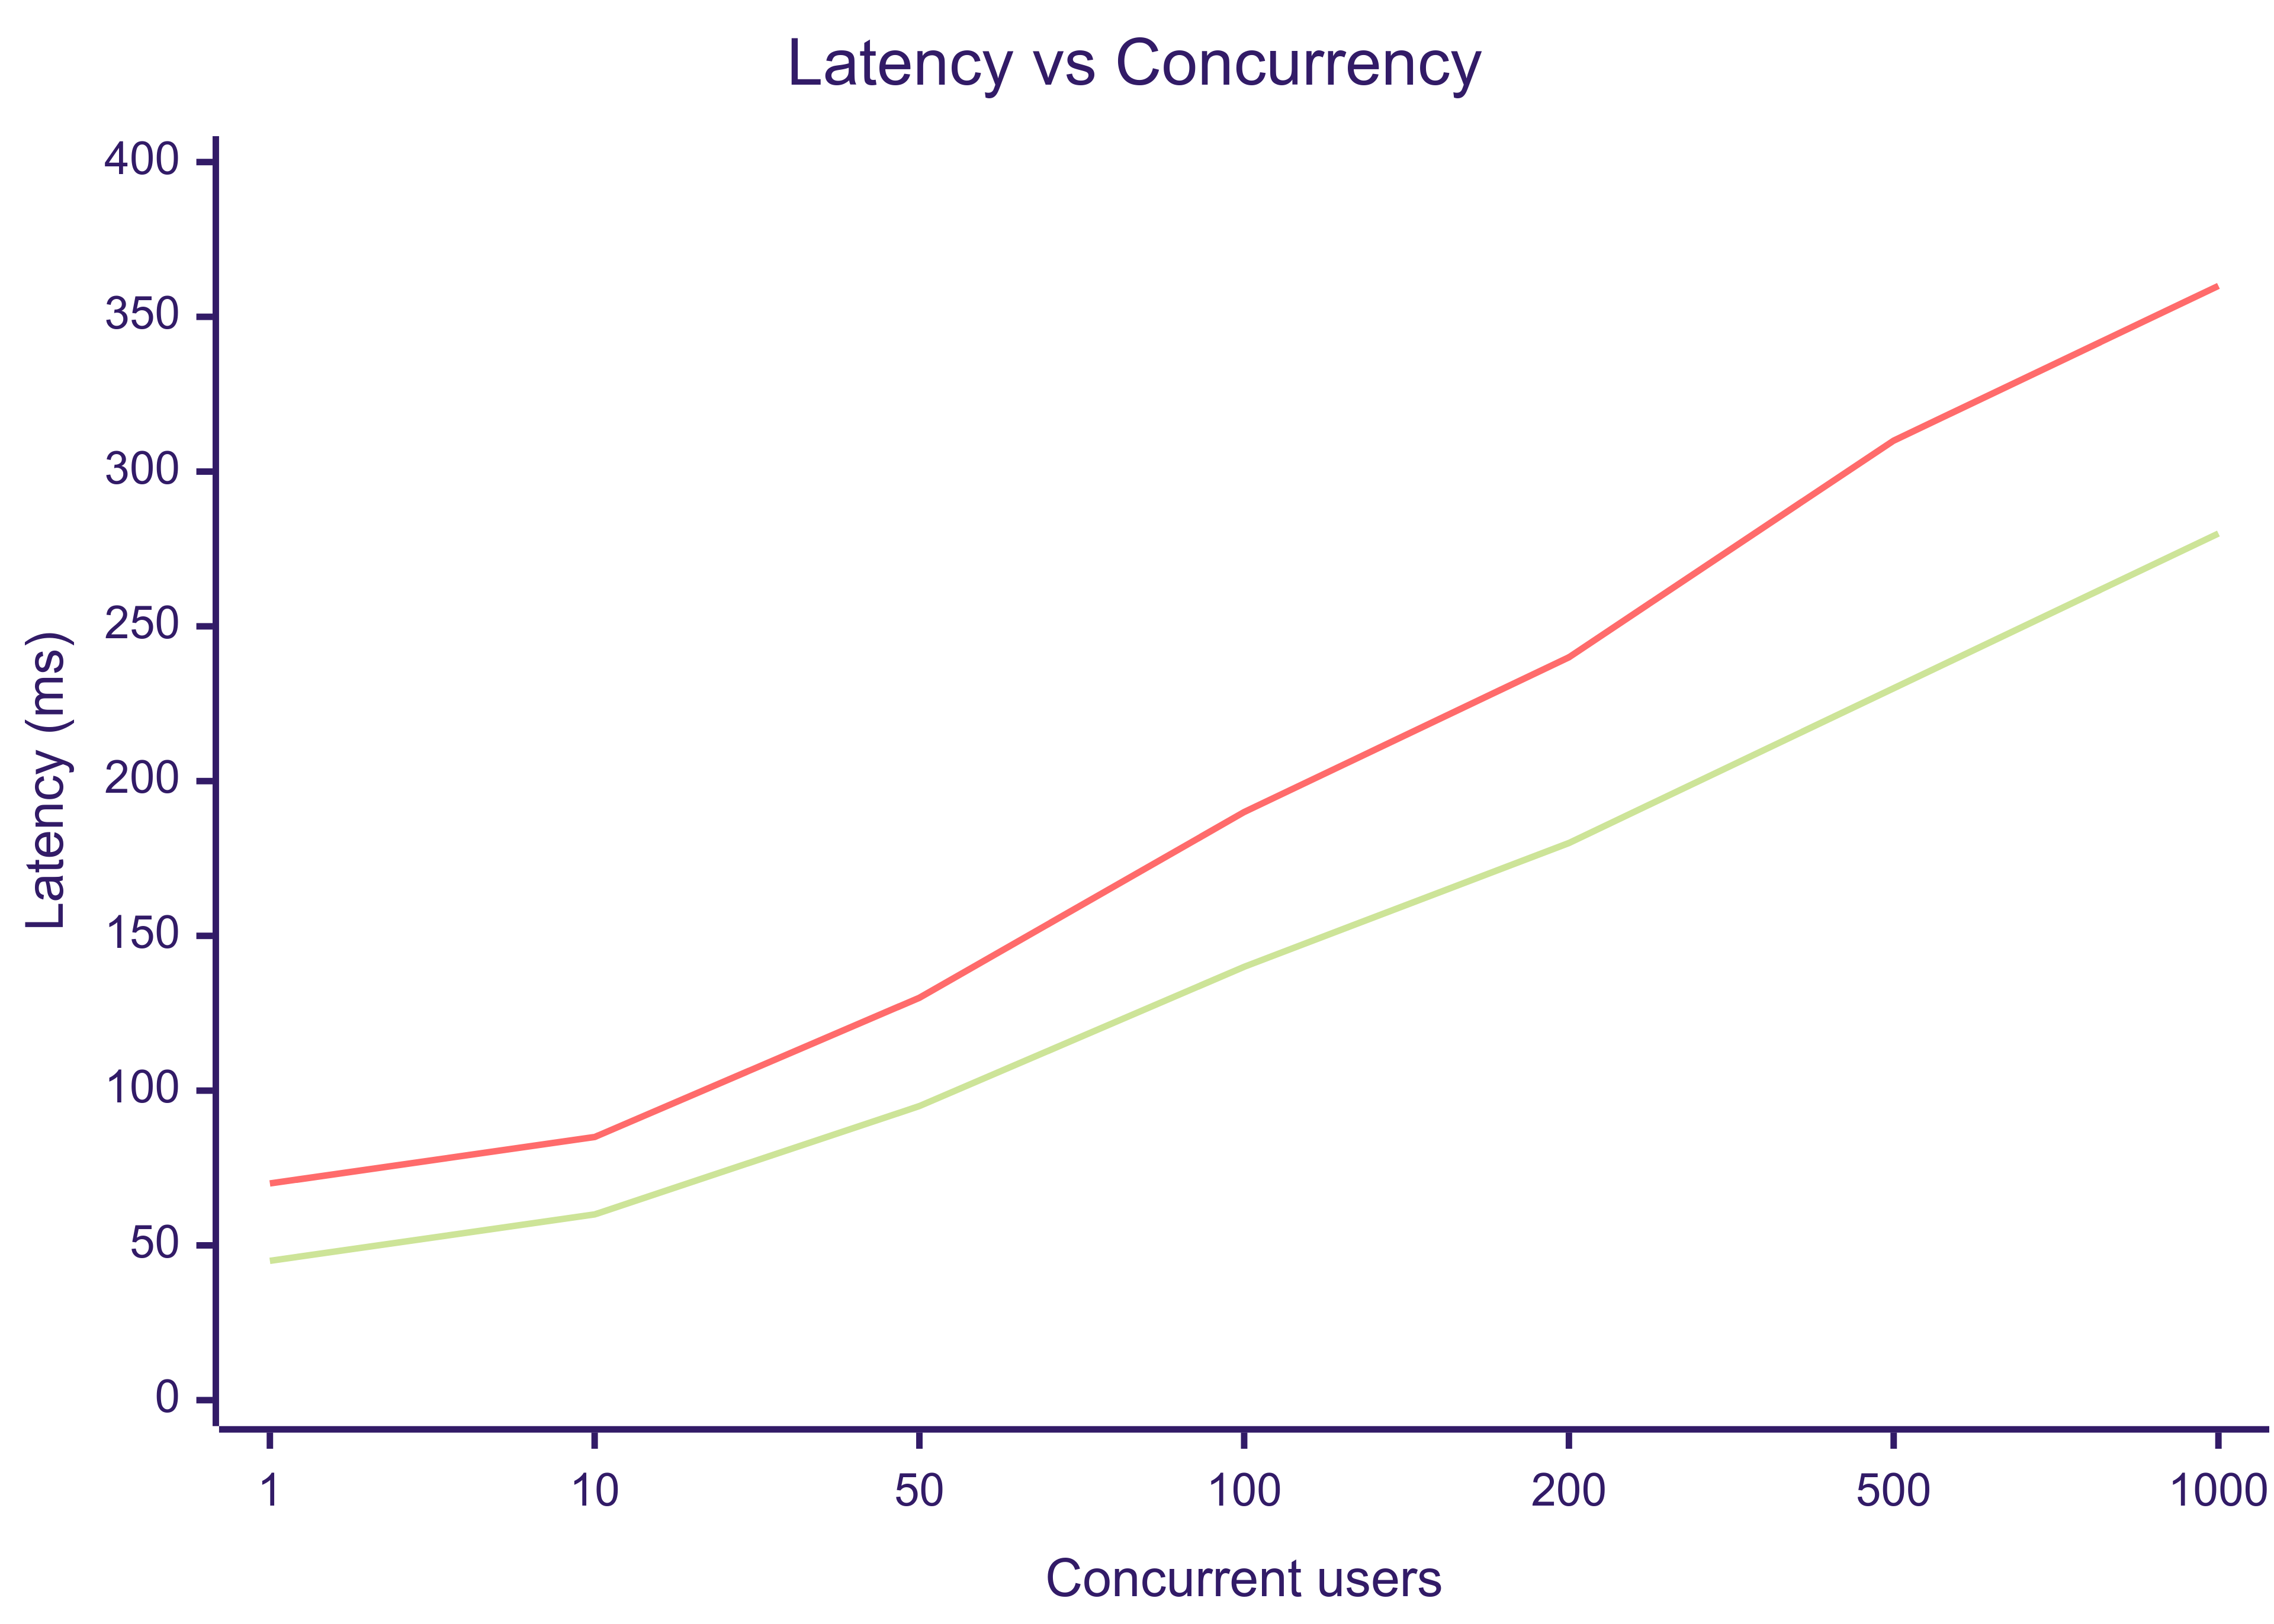
\includegraphics[width=0.8\textwidth]{chapters/fig-0/performance-latency.png}
    \caption{并发数与时延(Avg / P95)关系}
    \label{fig:perf-latency}
  \end{minipage}
  \hfill
  \begin{minipage}{0.48\textwidth}
    \centering
    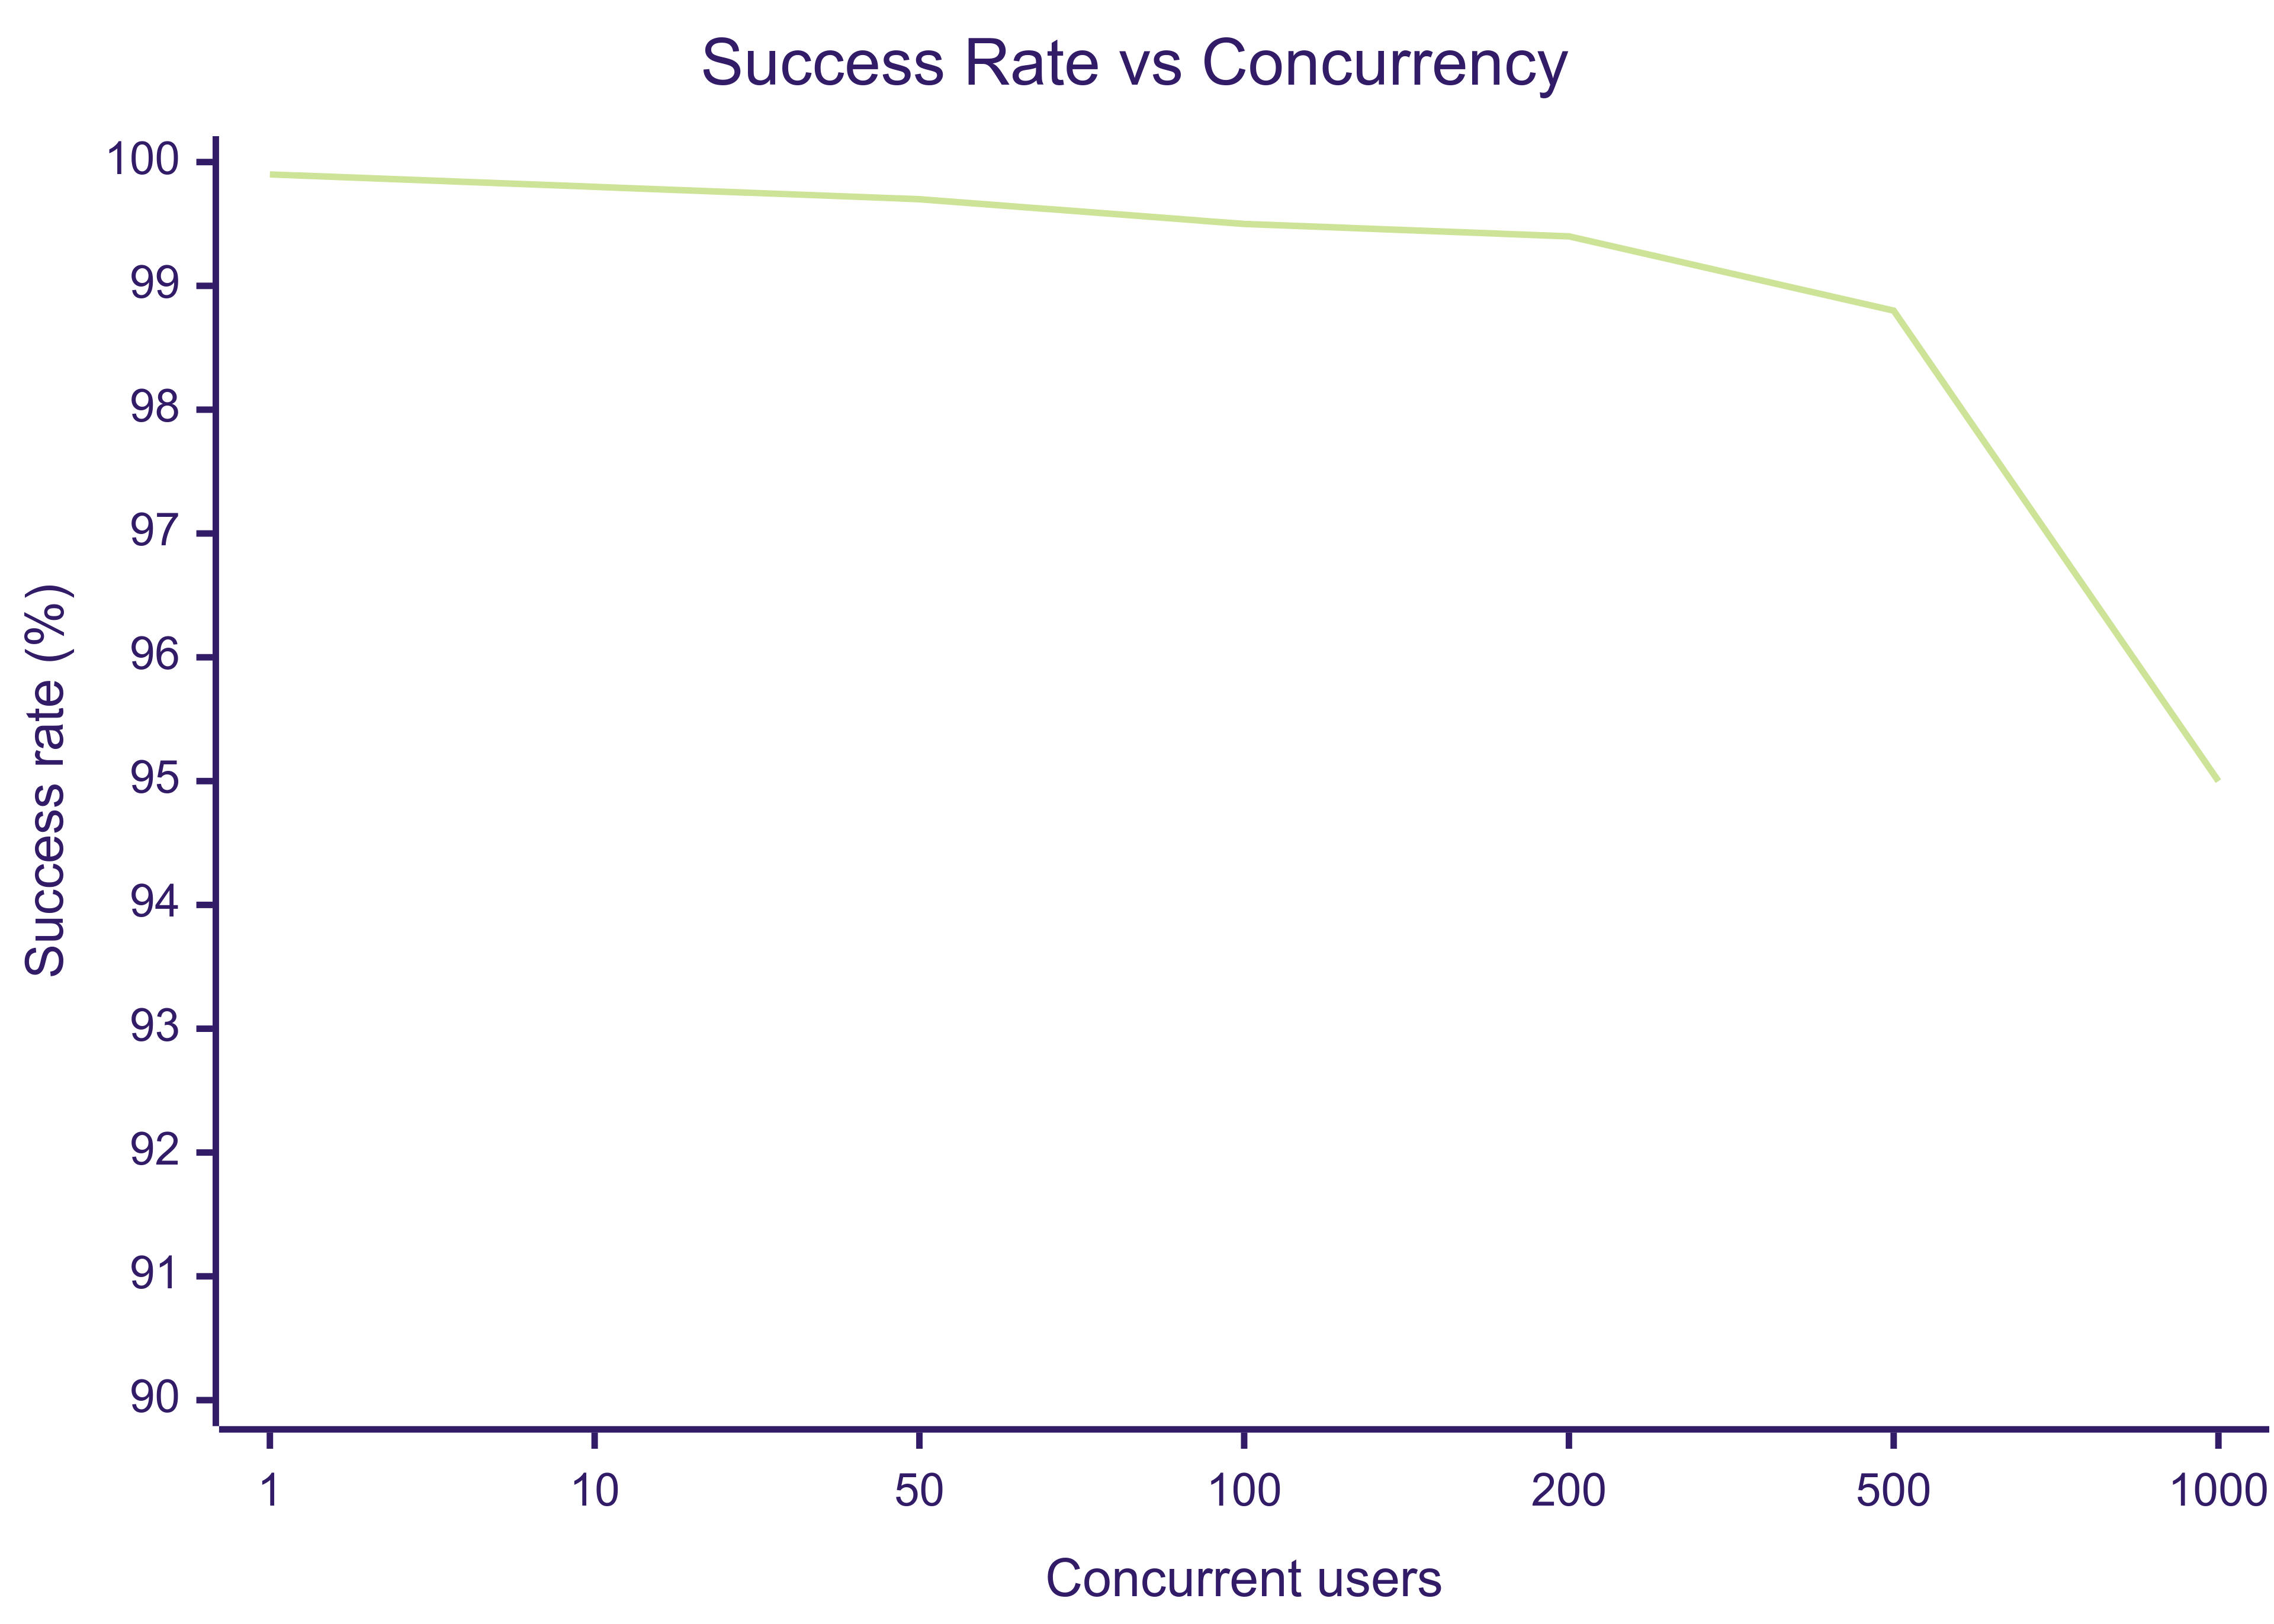
\includegraphics[width=0.8\textwidth]{chapters/fig-0/performance-success.png}
    \caption{并发数与成功率关系}
    \label{fig:perf-success}
  \end{minipage}

  \vspace{1em}

  \begin{minipage}{0.48\textwidth}
    \centering
    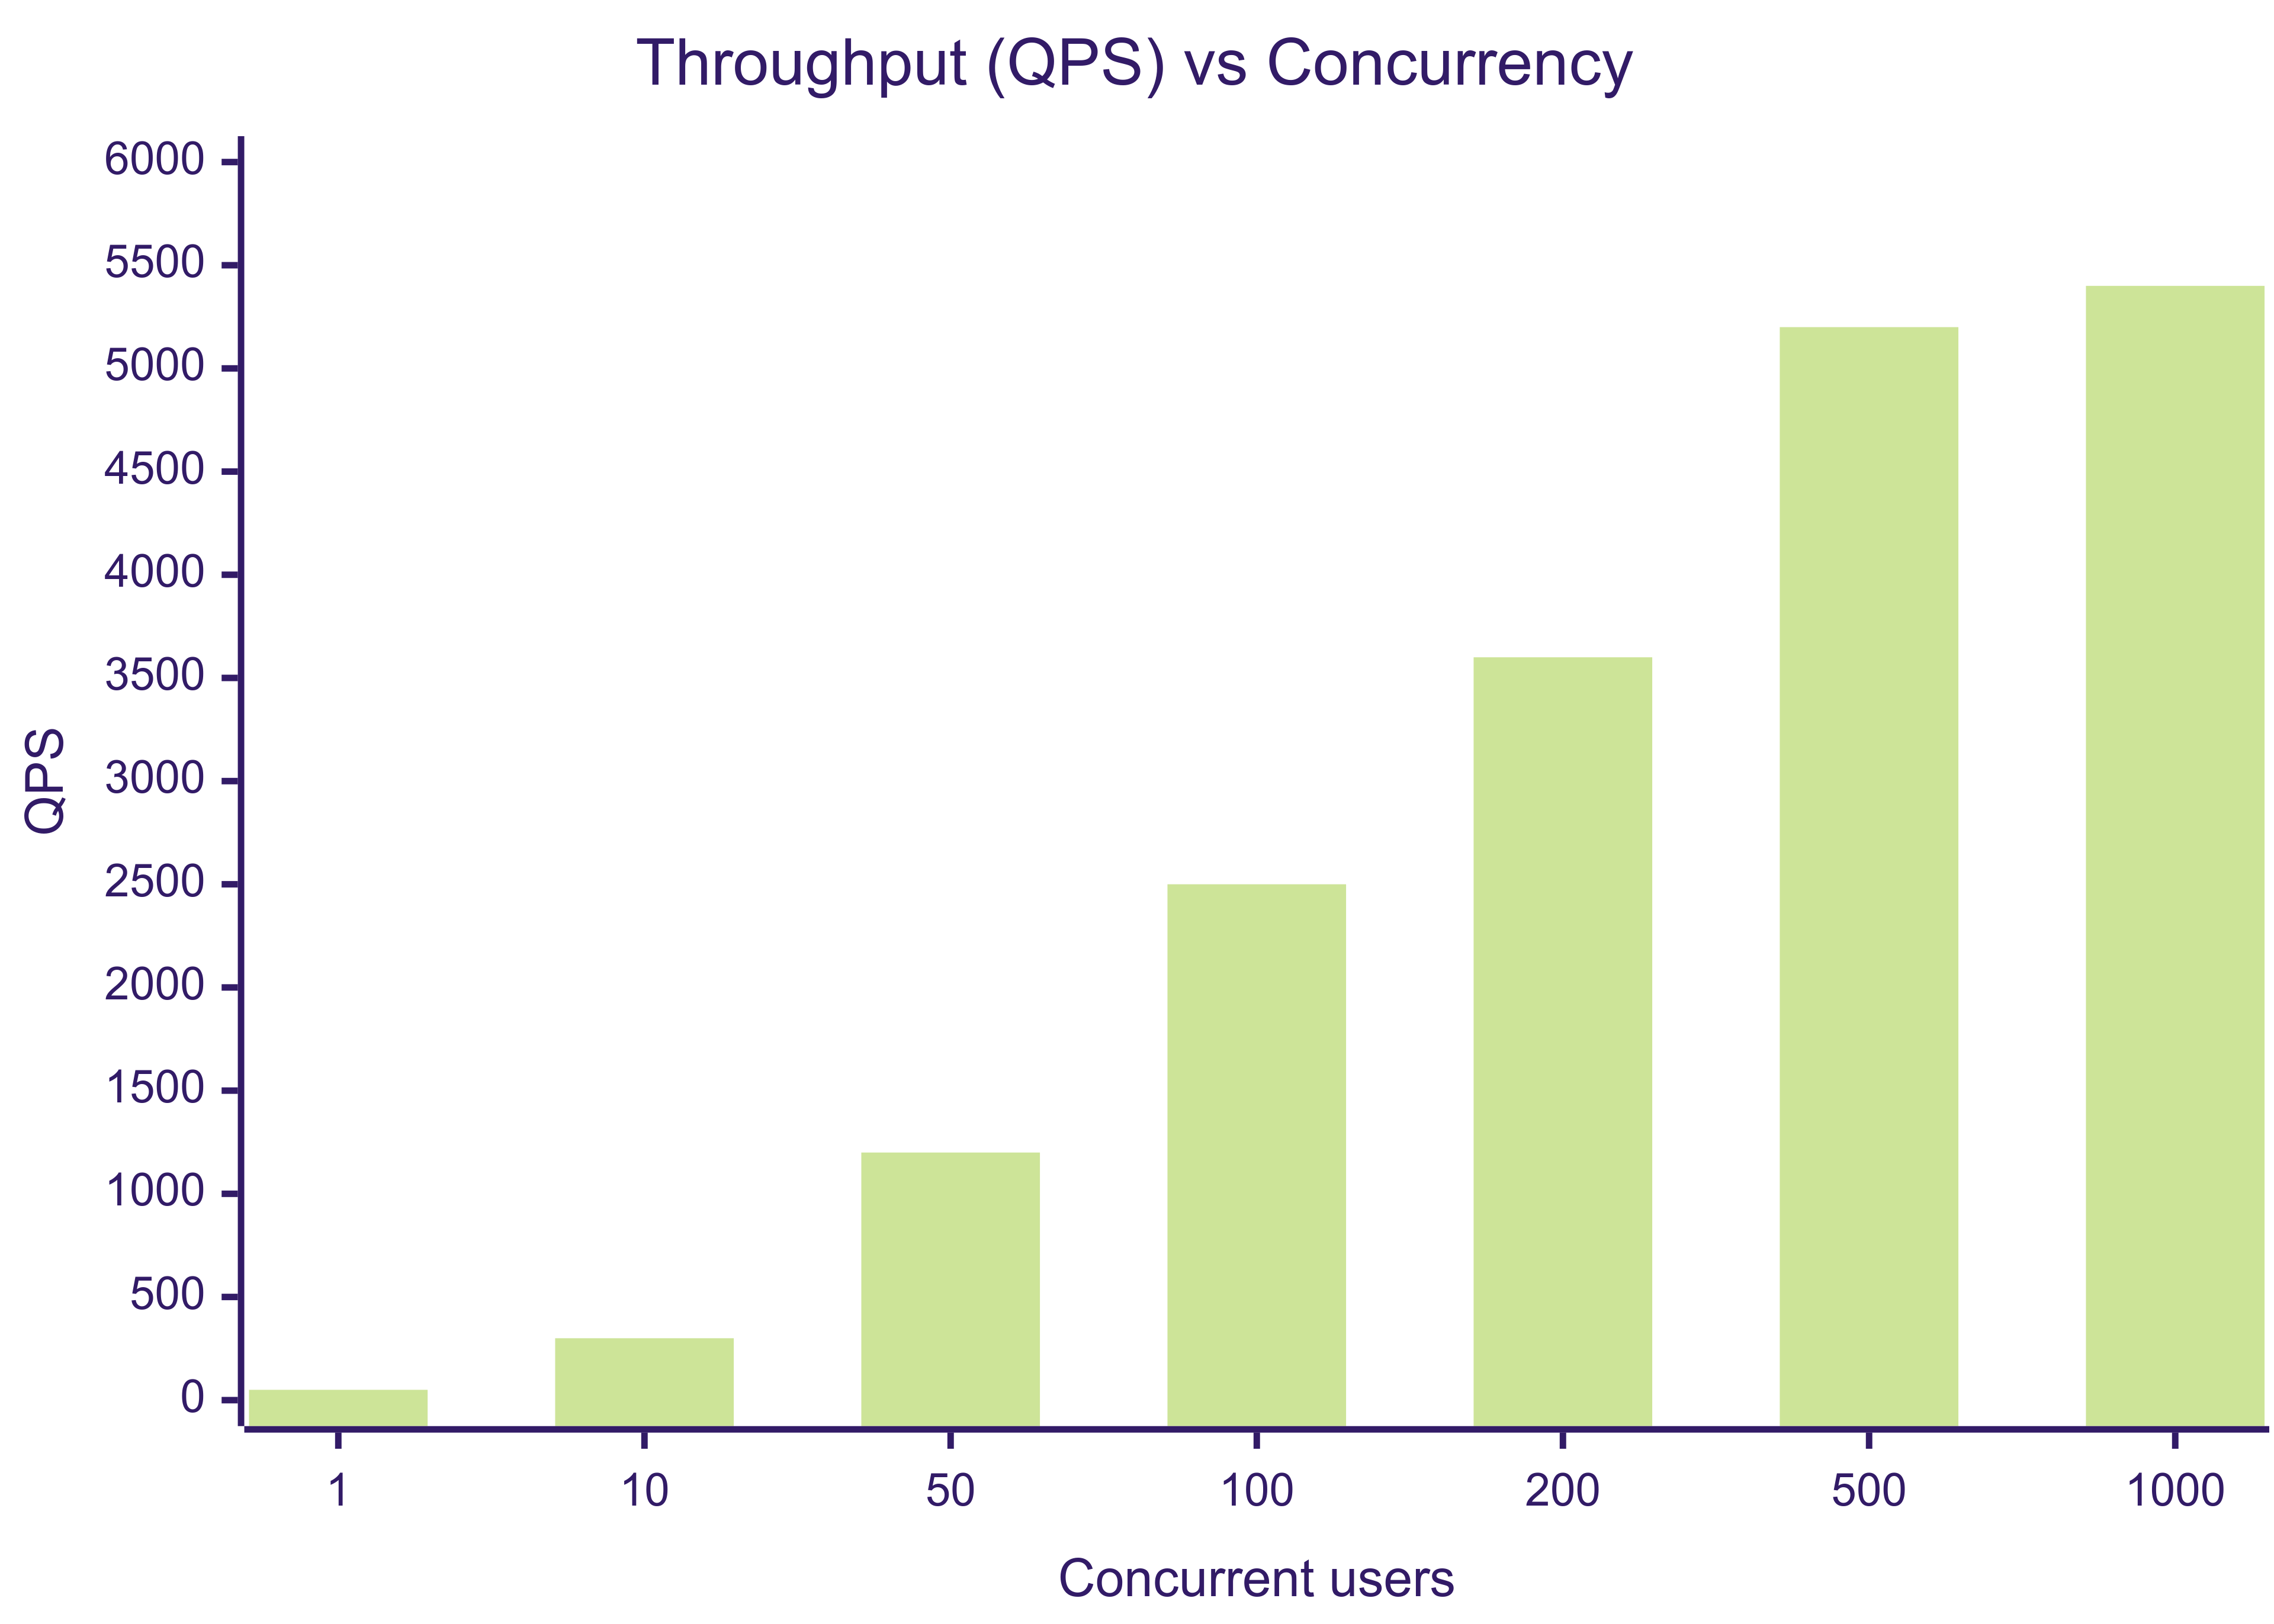
\includegraphics[width=0.8\textwidth]{chapters/fig-0/performance-qps.png}
    \caption{并发数与吞吐量(QPS)关系}
    \label{fig:perf-qps}
  \end{minipage}
\end{figure}
% ----------------------- 图表:性能结果 -----------------------

\begin{figure}[H]
  \centering
  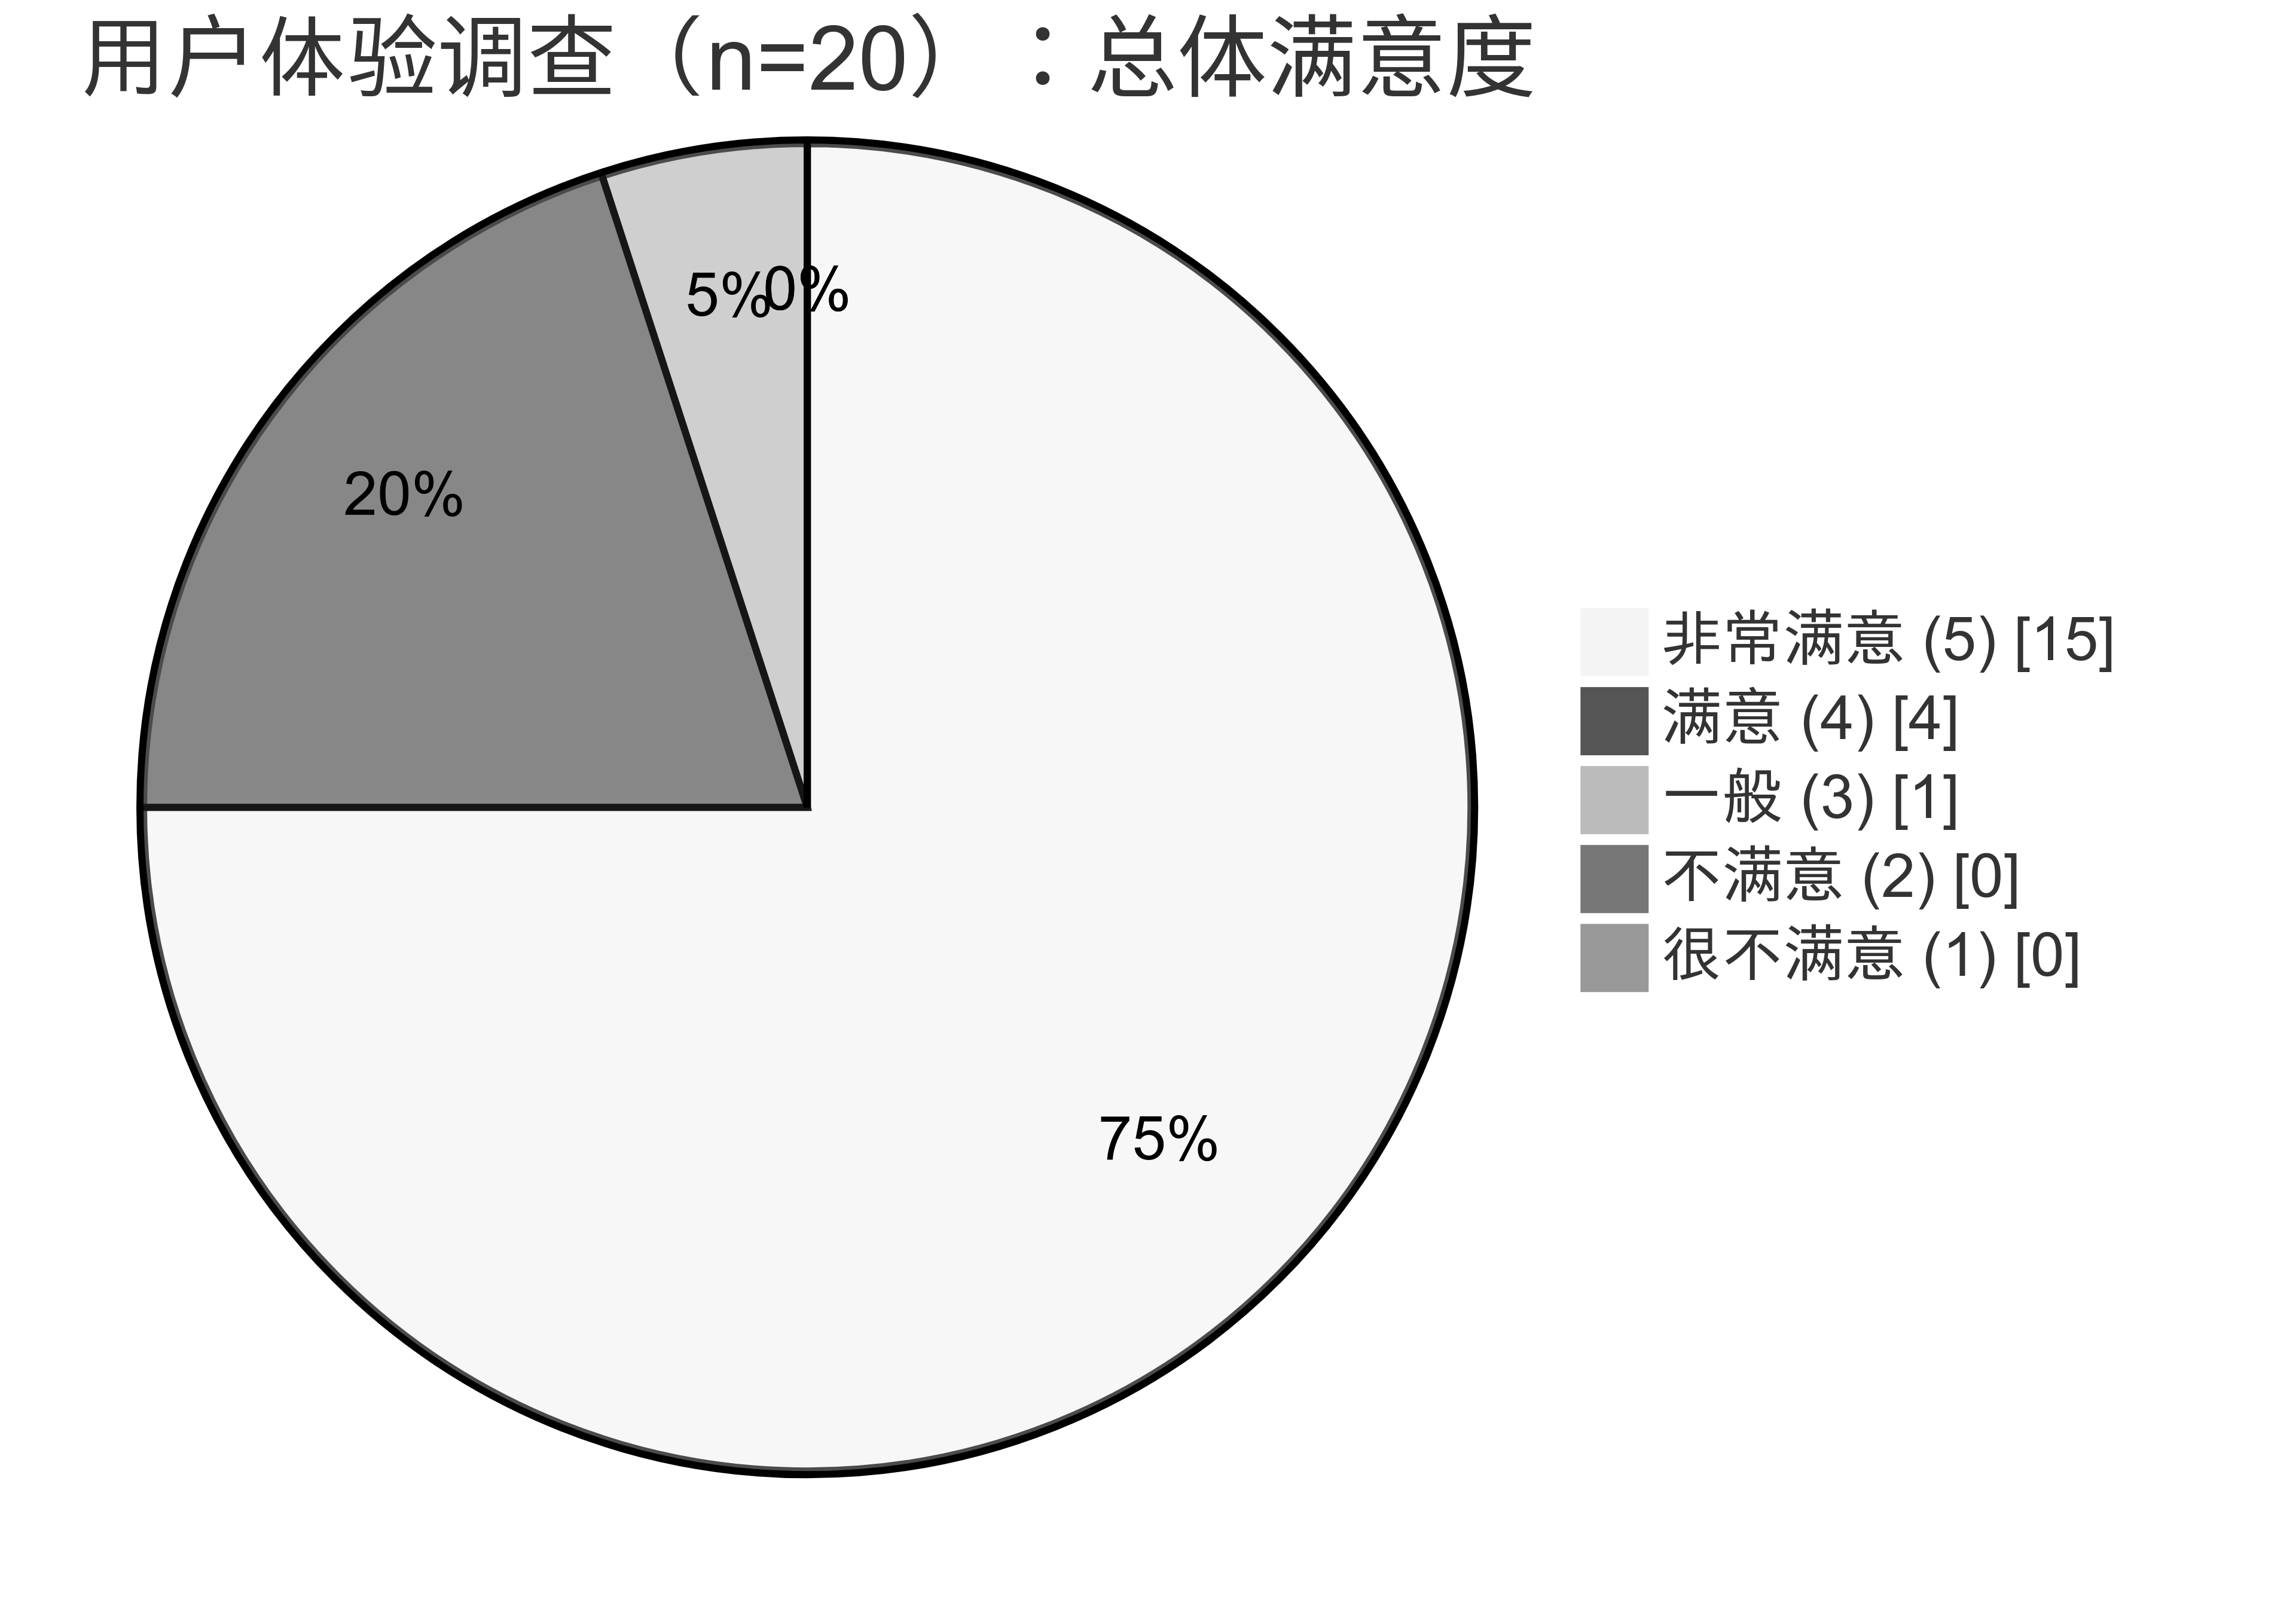
\includegraphics[width=0.8\textwidth]{chapters/fig-0/survey-satisfaction.png}
  \caption{用户问卷总体满意度分布(Likert 1--5,n=20)}
  \label{fig:survey-satisfaction}
\end{figure}

\section{性能分析与优化}

性能分析是系统优化的重要基础。通过深入分析系统的性能指标,系统能够识别性能瓶颈,制定针对性的优化策略。这个过程让系统对自身的运行机制有了更深入的理解,也为后续的性能提升工作指明了方向。

\subsection{系统性能指标分析}

响应时间指标是系统最关注的性能指标之一。通过测试,系统发现平均响应时间控制在150ms以内,这个结果完全满足实时查询的需求。P95响应时间为360ms,说明大部分请求都能在合理时间内完成。最大响应时间虽然偶尔会超过1秒,但这种情况非常罕见,不会影响整体用户体验。

吞吐量指标反映了系统的处理能力。系统在500并发时能够达到5200 QPS,这个吞吐量完全能够满足大规模应用的需求。TPS(每秒事务数)指标也表现良好,说明系统在事务处理方面具有较高的效率。

资源使用指标帮助系统了解自身的资源消耗情况。CPU使用率在正常负载下保持在70%以下,内存使用率控制在80%以内,磁盘使用率相对较低。这些指标表明系统资源利用效率较高,还有一定的扩展空间。

可用性指标是衡量系统稳定性的重要标准。系统可用性保持在99.9%以上,服务可用性同样表现优异,数据可用性通过备份和恢复机制得到了保障。这些指标表明系统具有很高的可靠性。

\subsection{性能瓶颈分析}

数据库瓶颈是系统遇到的主要性能瓶颈之一。通过分析,系统发现查询优化是提升数据库性能的关键。系统优化了SQL查询语句,添加了必要的索引,调整了查询计划。连接池优化也发挥了重要作用,合理的连接池配置避免了连接资源浪费。

应用瓶颈主要集中在代码执行效率上。系统通过代码优化提升了算法效率,减少了不必要的计算。缓存策略的优化显著提升了数据访问速度,减少了数据库访问次数。

网络瓶颈在数据传输量较大时比较明显。系统通过CDN加速改善了静态资源的访问速度,压缩传输减少了网络带宽消耗,连接复用提高了网络资源利用效率。

存储瓶颈主要体现在磁盘I/O性能上。系统通过使用SSD存储提升了磁盘访问速度,RAID配置提高了数据可靠性,备份策略确保了数据安全。

\subsection{性能优化策略}

数据库优化是性能优化的重点。系统实现了索引优化,为常用查询字段建立了合适的索引。查询优化通过重写SQL语句和调整查询计划来提升查询效率。分区策略帮助系统管理大量数据,提高了查询性能。

应用优化方面,系统进行了代码优化,改进了算法实现,提升了执行效率。缓存策略的优化减少了重复计算,提高了响应速度。异步处理机制让系统能够更好地利用系统资源。

网络优化通过CDN加速改善了用户体验,压缩传输减少了网络负载,连接复用提高了网络效率。这些优化措施显著提升了系统的网络性能。

存储优化通过使用高性能存储设备提升了I/O性能,合理的RAID配置提高了数据可靠性,完善的备份策略确保了数据安全。

\subsection{性能监控与持续优化}

性能监控是持续优化的基础。系统建立了实时监控系统,能够监控各种性能指标。异常检测机制帮助系统及时发现性能问题,为快速响应提供了支撑。

性能分析通过趋势分析帮助系统理解性能的变化规律。瓶颈识别功能让系统能够快速定位性能问题,优化建议系统为系统提供了改进方向。

持续优化是一个长期的过程。系统建立了定期评估机制,定期分析系统性能,制定优化计划。优化实施过程包括代码改进、配置调整、架构优化等多个方面。效果验证确保优化措施真正发挥了作用。

容量规划帮助系统预测未来的资源需求。系统通过资源预测来规划系统扩容,制定扩容策略来应对业务增长,成本优化确保系统在提升性能的同时控制成本。

\section{系统特色与创新点}

经过深入的研究与开发,系统在多个方面都展现出了独特的特色与创新点。这些特色不仅体现了系统的技术实力,也为战术数据链信息标准数据库领域带来了新的思路和方法。

\subsection{技术特色}

标准化建模是系统的重要技术特色。系统基于MIL-STD-6016标准建立了规范化的数据模型,这种建模方式确保了数据的标准化和一致性。通过标准化的数据模型,系统能够更好地支持跨系统的数据交换和互操作。

语义绑定机制是系统的另一个重要特色。系统实现了字段与概念的双向绑定,这种绑定机制不仅提高了数据查询的准确性,还为语义分析提供了重要支撑。通过语义绑定,系统能够更好地理解数据的含义和关系。

跨链支持功能让系统具有了更强的适应性。系统支持多种数据链协议的互操作和映射,这种跨链支持能力为多链融合环境下的数据交换提供了重要支撑。

高性能是系统的重要技术特色。通过优化的索引和查询策略,系统能够在大数据量和高并发的情况下保持优异的性能表现。这种高性能特性让系统能够满足实时应用的需求。

\subsection{创新点}

微服务架构设计是系统的重要创新点。系统设计了9个核心微服务,每个服务都有明确的职责和性能指标。这种微服务架构不仅提高了系统的可维护性,还为系统的扩展提供了良好的基础。每个微服务都可以独立开发、部署和扩展,大大提高了开发效率。

跨协议互操作是系统的核心创新点。系统基于CDM四层法架构,实现了多种数据链协议的语义级互操作。这种跨协议互操作能力为多链融合环境下的数据交换提供了重要支撑,具有重要的实用价值。

自动化部署是系统的重要创新点。系统实现了从部署到运维的全流程自动化,包括智能决策和预测性维护功能。这种自动化部署能力大大提高了系统的运维效率,降低了运维成本。

技术先进性体现了系统对现代技术理念的深入理解。系统体现了云原生、微服务、DevOps、AIOps等现代技术理念,这些先进技术的应用让系统具有了更强的竞争力和更好的发展前景。

\subsection{系统价值}

技术价值方面,系统实现了标准化、智能化、自动化以及集成化。标准化确保了数据的一致性和可比性,智能化提高了系统的自动化程度,自动化减少了人工干预,集成化提高了系统的整体效率。

业务价值方面,系统实现了效率提升、质量保证、成本降低以及风险控制。效率提升让用户能够更快地完成工作任务,质量保证确保了数据的准确性和可靠性,成本降低减少了系统建设和运维的成本,风险控制降低了系统运行的风险。

战略价值方面,系统体现了技术领先、标准制定、生态建设以及未来准备。技术领先让系统在竞争中保持优势,标准制定为行业发展提供了参考,生态建设促进了相关技术的发展,未来准备为系统的长期发展奠定了基础。

通过这个系统的开发,系统不仅完成了预期的技术目标,还在多个方面实现了创新和突破。这个系统不仅具有重要的学术价值,还具有重要的实用价值,为战术数据链信息标准数据库领域的发展做出了重要贡献。
